\documentclass[11pt, a4paper, oneside]{amsart}

\title{The Pigeonhole Principle}
\date{Last updated : \today}
\author{Jonathan Prieto-Cubides}


% ================================================================

\usepackage{fontspec,xltxtra,xunicode}
\usepackage[warnings-off={mathtools-colon,%
                          mathtools-overbracket}
            ]{unicode-math}
\defaultfontfeatures{Ligatures=TeX}
\setmonofont[Mapping=tex-text]{PragmataPro Mono}

% ================================================================
\usepackage{graphicx,overpic}

\usepackage[usenames,dvipsnames]{xcolor}
\definecolor{obj1}{rgb}{.88,, .93,, .96}
\definecolor{obj2}{rgb}{.62,, .74,, .85}
\definecolor{obj3}{rgb}{.53,, .34, .65}
\definecolor{obj4}{rgb}{.74,, .74, .74}

\newcommand\myshade{85}
\colorlet{mylinkcolor}{violet}
\colorlet{mycitecolor}{YellowOrange}
\colorlet{myurlcolor}{Aquamarine}

\definecolor{refkey}{gray}{.75}
\definecolor{labelkey}{gray}{.75}
% ================================================================

\usepackage{adjustbox}

\newenvironment{shade}{%
%
\vskip 0.1\baselineskip%
\begin{adjustbox}{%
minipage=\linewidth,margin=0pt,padding=0pt,bgcolor=obj1%
}}{%
\end{adjustbox}%
\vskip 0.1\baselineskip%
%
}
% ================================================================
\usepackage{graphicx}
\graphicspath{{./../docs/ipe-images/}}

\usepackage[color=obj1]{todonotes}
\usepackage{wrapfig}

\usepackage{url}

\usepackage{enumerate}
\usepackage[shortlabels]{enumitem}
\usepackage[yyyymmdd,hhmmss]{datetime}

% =================================================================

\usepackage{amsmath, amsfonts, textcomp, mathtools, xparse}
% \usepackage{stmaryrd}
\usepackage{thmtools}
\usepackage{thm-restate}

\declaretheoremstyle[headfont=\normalfont\bfseries,bodyfont=\normalfont]{p-thm}
\declaretheoremstyle[headfont=\normalfont\bfseries]{p-def}

\declaretheorem[parent=section,style=p-thm]{theorem}
\declaretheorem[sibling=theorem,style=p-thm]{lemma}
\declaretheorem[sibling=theorem,style=p-thm]{proposition}
\declaretheorem[sibling=theorem,style=p-thm]{corollary}
\declaretheorem[sibling=theorem,style=p-thm]{conjecture}
\declaretheorem[sibling=theorem,style=p-thm]{axiom}
\declaretheorem[sibling=theorem,style=p-thm]{construction}
\declaretheorem[sibling=theorem,style=p-thm]{definition}
\declaretheorem[sibling=theorem,style=p-thm]{remark}
\declaretheorem[sibling=theorem,style=p-thm]{example}
\declaretheorem[sibling=theorem,style=p-thm]{exercise}

\let\oldproofname=\proofname
\renewcommand{\proofname}{\rm\bf{\oldproofname}}

\numberwithin{equation}{section}

\usepackage[all]{xy}
\usepackage{pgfplots,tikz, tikz-cd}
\pgfplotsset{compat=newest,compat/show suggested version=false}
\usetikzlibrary{decorations.markings,
decorations.pathreplacing,
matrix,
arrows,
chains,
positioning,scopes}

% ================================================================
% MACROS

\newcommand{\Agda}[0]{\textsf{Agda}}
\newcommand{\Aut}{\mathsf{Aut}}
\newcommand{\A}{\ensuremath{\texttt{A}}}
\newcommand{\Cn}{\ensuremath{\texttt{C}_{n}}}
\newcommand{\CombinatorialMap}{\ensuremath{\texttt{Map}}}
\newcommand{\CyclicGraph}{\ensuremath{\texttt{CyclicGraph}}}
\newcommand{\CyclicOrder}{\ensuremath{\texttt{CyclicOrder}}}
\newcommand{\DNE}{\ensuremath{\operatorname{DNE}}}
\newcommand{\EdgeIsProp}{\ensuremath{\mathsf{Edge-is-prop}}}
\newcommand{\Edge}{\ensuremath{\texttt{E}}}
\newcommand{\Embedding}{\ensuremath{\texttt{Embedding}}}
\newcommand{\Empty}{\mathbf{0}}
\newcommand{\Face}{\ensuremath{\texttt{Face}}}
\newcommand{\Fin}[1]{\ensuremath{\mathsf{Fin}_{#1}}}
\newcommand{\Graph}{\ensuremath{\texttt{Graph}}}
\newcommand{\IsUndirected}{\ensuremath{\texttt{Undirected}}}
\newcommand{\IsSimple}{\ensuremath{\texttt{IsSimple}}}
\newcommand{\HoTT}[0]{\textsf{HoTT}}
\newcommand{\Hom}[2]{\ensuremath{\mathsf{Hom}({#1},{#2})}}
\newcommand{\IsoHom}[1]{\ensuremath{\mathsf{IsoHom}\,{#1}}}
\newcommand{\Iso}[2]{\ensuremath{#1\simeq_{\texttt{Iso}}#2}}
\newcommand{\LEM}{\ensuremath{\operatorname{LEM}}}
\newcommand{\NodeIsSet}{\ensuremath{\mathsf{NodeIsSet}}}
\newcommand{\Node}{\ensuremath{\texttt{N}}}
\newcommand{\N}{\mathbb{N}}
\newcommand{\PathOver}{\operatorname{PathOver}}
\newcommand{\Path}{\ensuremath{\mathsf{Path}}}
\newcommand{\Planar}{\texttt{Planar}}
\newcommand{\Rotation}{\texttt{Rotation}}
\newcommand{\RS}{\ensuremath{\mathsf{R}}}
\newcommand{\R}{\ensuremath{\texttt{R}}}
\newcommand{\Set}{\operatorname{Set}}
\newcommand{\Spherical}{\ensuremath{\texttt{Spherical}}}
\newcommand{\Star}{\ensuremath{\mathtt{Star}}}
\newcommand{\hSet}{\ensuremath{\mathsf{hSet}}}
\newcommand{\hProp}{\ensuremath{\mathsf{hProp}}}
\newcommand{\Type}{\ensuremath{\mathsf{Type}}}
\newcommand{\UU}{\mathcal{U}}
\newcommand{\VV}{\mathcal{V}}
\newcommand{\Walk}{\ensuremath{\texttt{Walk}}}
\newcommand{\ap}{\operatorname{ap}}
\newcommand{\bool}{\mathbf{2}}
\newcommand{\bracket}[1]{\left( #1 \right)}
\newcommand{\coe}{\operatorname{coe}}
\newcommand{\comp}{\mathrel{\circ}}
\newcommand{\false}{\operatorname{false}}
\newcommand{\flip}{\operatorname{flip}}
\newcommand{\fun}{\operatorname{fun}}
\newcommand{\idfunc}[1][]{\operatorname{id}_{#1}}
\newcommand{\id}{\operatorname{id}}
\newcommand{\ind}{\operatorname{ind}}
\newcommand{\inl}{{\operatorname{inl}}}
\newcommand{\inr}{{\operatorname{inr}}}
\newcommand{\isContr}[1]{\ensuremath{\mathsf{isContr}(#1)}}
\newcommand{\isPlanar}{\operatorname{isPlanar}}
\newcommand{\isProp}[1]{\ensuremath{\mathsf{isProp}(#1)}}
\newcommand{\isSet}[1]{\ensuremath{\mathsf{isSet}(#1)}}
\newcommand{\pr}{\operatorname{pr}}
\newcommand{\rec}{\operatorname{rec}}
\newcommand{\refl}{\operatorname{refl}}
\newcommand{\sym}{\operatorname{sym}}
\newcommand{\transport}{\operatorname{trans}}
\newcommand{\trdos}[5]{\ensuremath{\mathsf{tr}_{2}^{#1,#2}(#3,#4,#5)}}
\newcommand{\true}{\operatorname{true}}
\newcommand{\trunc}[1]{\left\|\,#1\,\right\|}
\newcommand{\tr}[3]{\ensuremath{\mathsf{tr}^{#1}(#2,#3)}}
\newcommand{\ttt}{\star}
\newcommand{\unit}{\mathbf{1}}
\renewcommand{\equiv}{\simeq}

\usepackage[
  unicode=true,
  bookmarks=true,
  % %
  linkcolor  = mylinkcolor!\myshade!black,
  citecolor  = obj4,
  urlcolor   = myurlcolor!\myshade!black,
  colorlinks = true,
  % %
  pdftitle={Univalent Graphs},
  pdfauthor={Jonathan Prieto-Cubides and Håkon Robbestad Gylterud},
  breaklinks=true,
  pdfencoding=auto
  ]{hyperref}

\usepackage[capitalize]{cleveref}

% ================================================================

% \usepackage[notref,notcite,color]{showkeys}
\usepackage{latex/agda}

\begin{document}

\maketitle

\begin{abstract}
There are many formulations of the so-called Pigeonhole principle,
some of them proved in constructive mathematics and formalized
in some proof-assistants. In this work, we show one these formulations
proved in the context of Univalent Type theory and
formalized in the proof-assistant Agda.
\end{abstract}

\section{Introduction}

The pigeonhole principle says that \emph{if you put $n$ pigeons in
$m$ holes, with $m < n$, then at least one hole has more
than one pigeon in it.
}\\

In~\cite{symmetrybook} the authors give the following formulation
(\Cref{lem:PHP}) of the Pigeonhole Principle joint with a constructive proof
that it holds. The proof can be found formalized in \texttt{Coq}\footnote{In
the \texttt{Coq} standard library
\url{https://coq.inria.fr/library/Coq.Sets.Image.html}.}.

\begin{theorem}[Lemma 2.15.6 in \cite{symmetrybook}]\label{lem:PHP}
For all $N:ℕ$ and $f:ℕ\to ℕ$ such that $f(n)<N$
for all $n<N+1$, there exist $m < n < N+1$ such that $f(n)=f(m)$.
\end{theorem}
The function $f$ above intends to maps the number of a pigeon in $\{0\cdots n−1\}$ to
the number of its hole in $\{0\cdots m−1\}$.

In this work, we consider an equivalent formulation in \Cref{pigeon-theorem},
which can be seen as a generalization of \Cref{lem:PHP}. The formal statement
says, there is no injective function that can go from a finite set to a smaller
one. We denote the finite set of $n$ elements with $[n]$.

\begin{theorem}[Pigeonhole Theorem]\label{pigeon-theorem}
For any $n,\, m : ℕ$ when $m < n$,  a function $f : [ n ] \to [ m ]$
can not be injective.
\end{theorem}

Another similar formulation can be stated when instead of finite sets, we
consider for any function, the cardinality of its domain and its image. We
give the following formulations that follow the same fashion of
\Cref{pigeon-theorem}.

For any $n : ℕ$, $f : [n] \to [n]$.
\begin{itemize}
\item If $f$ is a surjective, then $f$ is injective, and
\item If $f$ is injective, then $f$ is surjective.
\end{itemize}

\section{Notation}

\subsection{Agda formalization}

To check the proof in~\Cref{proof-pigeon-theorem} of \Cref{pigeon-theorem}, we
use \texttt{Agda v2.6.0} without the \emph{Axiom K} to be consistent with
Univalent mathematics. We also import a library to work with Homotopy Type
Theory called \texttt{MiniHoTT}\footnote{Available on
\url{http://jonaprieto.github.io/mini-hott}.} that includes some type
definitions and theorems we need.

\begin{code}%
\>[0]\AgdaSymbol{\{-\#}\AgdaSpace{}%
\AgdaKeyword{OPTIONS}\AgdaSpace{}%
\AgdaPragma{--without-K}%
\>[25]\AgdaSymbol{\#-\}}\<%
\\
\>[0]\AgdaKeyword{open}\AgdaSpace{}%
\AgdaKeyword{import}\AgdaSpace{}%
\AgdaModule{MiniHoTT}\<%
\end{code}

\begin{code}[hide]%
\>[0][@{}l@{\AgdaIndent{1}}]%
\>[2]\AgdaKeyword{hiding}\AgdaSpace{}%
\AgdaSymbol{(}\AgdaOperator{\AgdaFunction{⟦\AgdaUnderscore{}⟧}}\AgdaSymbol{)}\<%
\\
\>[0]\AgdaKeyword{module}\AgdaSpace{}%
\AgdaModule{\AgdaUnderscore{}}\AgdaSpace{}%
\AgdaSymbol{\{}\AgdaBound{ℓ}\AgdaSpace{}%
\AgdaSymbol{:}\AgdaSpace{}%
\AgdaPostulate{Level}\AgdaSymbol{\}}\AgdaSpace{}%
\AgdaKeyword{where}\<%
\\
\>[0][@{}l@{\AgdaIndent{0}}]%
\>[2]\AgdaKeyword{open}\AgdaSpace{}%
\AgdaModule{ℕ-ordering}\AgdaSpace{}%
\AgdaBound{ℓ}\<%
\\
%
\>[2]\AgdaOperator{\AgdaFunction{⟦\AgdaUnderscore{}⟧}}\AgdaSpace{}%
\AgdaSymbol{=}\AgdaSpace{}%
\AgdaOperator{\AgdaFunction{⟦\AgdaUnderscore{}⟧₂}}\AgdaSpace{}%
\AgdaSymbol{\{}\AgdaBound{ℓ}\AgdaSymbol{\}}\<%
\end{code}

\subsection{Types}

We assume the reader is familiar with type theory notation as in Book HoTT
\cite{hottbook} and with the basic \Agda\, syntax. For any type $A : \Type$,
we define in~\Cref{eq:minus} the type $A - \{x\}$ as the type\footnote{We
denote this symbol, minus, as  double-back-slashes in \Agda.} of elements of
which are different with $x$. We will use this type to talk about the finite
set $[n]$ without a point $x$, i.e., $[n] - \{ x\}$. The finite set of $n$
elements in \texttt{Agda} is denoted by \texttt{⟦ n ⟧}. We are using for
finite sets the definition that says $[n + 1] :\equiv 𝟙 + [n]$ and $[0]
:\equiv 𝟘$. Propositional equality is denoted by ($\equiv$) instead of $(=)$.
The type $ℕ$ for natural numbers has two constructors \texttt{zero}, and
\texttt{succ}. The coproduct of types $A$ and $B$ is denoted by $A+B$ and it
has two introduction rules named \texttt{inr}, and \texttt{inl}. We use the
direct composition of functions also called \emph{diagramatic} composition,
denoted in \texttt{Agda} by (\texttt{f :> g}) for $f : A \to B$ and $g : B \to
C$, for types $A,B,$ and $C$.

\begin{equation}\label{eq:minus}
A - \{x\} :\equiv \sum_{a : A} \, (a ≡ x) → \bot.
\end{equation}

\begin{code}[hide]%
%
\>[2]\AgdaOperator{\AgdaFunction{\AgdaUnderscore{}─\AgdaUnderscore{}}}%
\>[7]\AgdaSymbol{:}\AgdaSpace{}%
\AgdaSymbol{∀}\AgdaSpace{}%
\AgdaSymbol{\{}\AgdaBound{ℓ}\AgdaSpace{}%
\AgdaSymbol{:}\AgdaSpace{}%
\AgdaPostulate{Level}\AgdaSymbol{\}}\AgdaSpace{}%
\AgdaSymbol{→}\AgdaSpace{}%
\AgdaSymbol{(}\AgdaBound{A}\AgdaSpace{}%
\AgdaSymbol{:}\AgdaSpace{}%
\AgdaFunction{Type}\AgdaSpace{}%
\AgdaBound{ℓ}\AgdaSymbol{)}\AgdaSpace{}%
\AgdaSymbol{(}\AgdaBound{x}\AgdaSpace{}%
\AgdaSymbol{:}\AgdaSpace{}%
\AgdaBound{A}\AgdaSymbol{)}\AgdaSpace{}%
\AgdaSymbol{→}\AgdaSpace{}%
\AgdaFunction{Type}\AgdaSpace{}%
\AgdaBound{ℓ}\<%
\\
%
\>[2]\AgdaOperator{\AgdaFunction{\AgdaUnderscore{}─\AgdaUnderscore{}}}%
\>[7]\AgdaSymbol{\{}\AgdaBound{ℓ}\AgdaSymbol{\}}\AgdaSpace{}%
\AgdaBound{A}\AgdaSpace{}%
\AgdaBound{x}%
\>[16]\AgdaSymbol{=}\AgdaSpace{}%
\AgdaRecord{∑}\AgdaSpace{}%
\AgdaBound{A}\AgdaSpace{}%
\AgdaSymbol{(λ}\AgdaSpace{}%
\AgdaBound{a}\AgdaSpace{}%
\AgdaSymbol{→}\AgdaSpace{}%
\AgdaSymbol{((}\AgdaBound{a}\AgdaSpace{}%
\AgdaOperator{\AgdaFunction{≡}}\AgdaSpace{}%
\AgdaBound{x}\AgdaSymbol{)}\AgdaSpace{}%
\AgdaSymbol{→}\AgdaSpace{}%
\AgdaFunction{⊥}\AgdaSpace{}%
\AgdaBound{ℓ}\AgdaSymbol{))}\<%
\end{code}

\section{A proof of \Cref{pigeon-theorem}}

We first need to show there exists an equivalence between two (finite) types
that differs only by one point. So we define the following (recursive)
functions \texttt{e→} and \texttt{e←}.

\begin{figure}
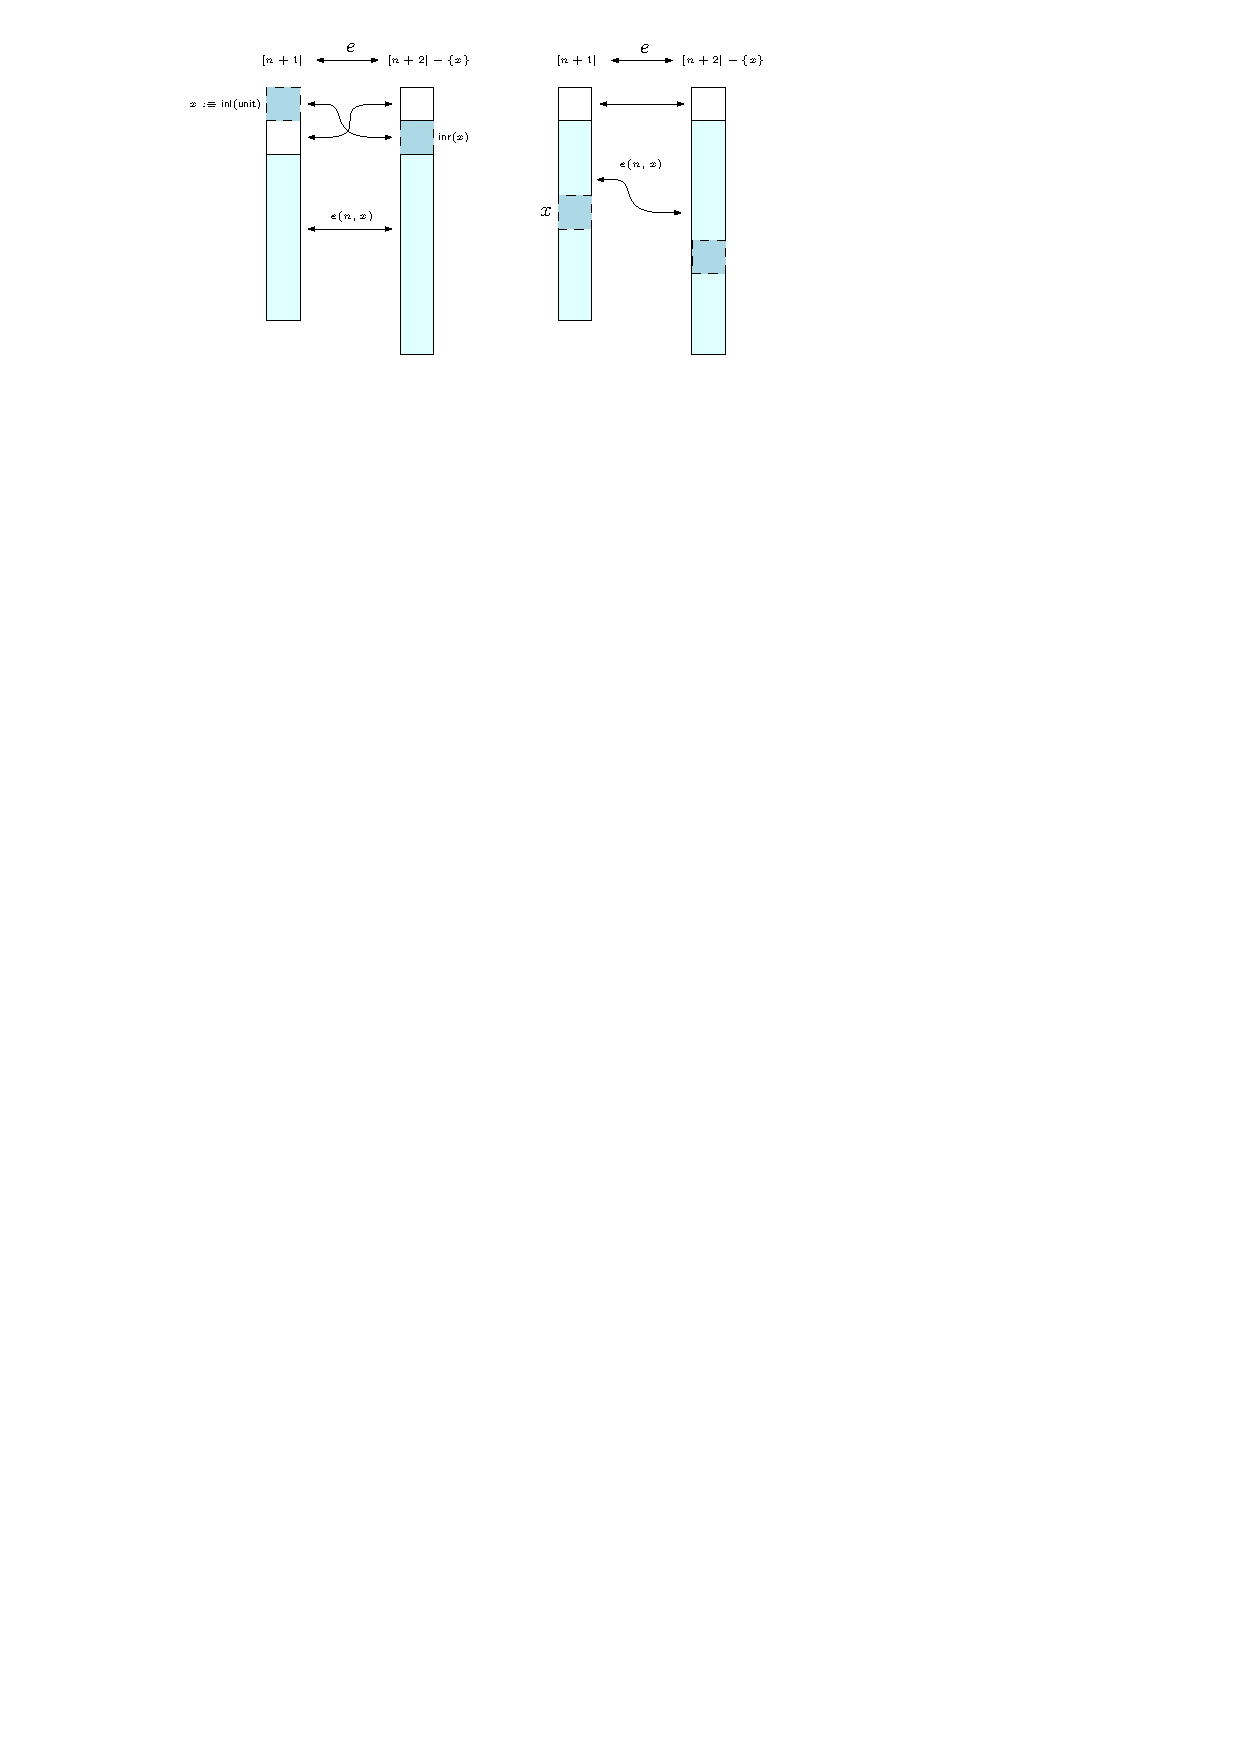
\includegraphics[width=0.9\textwidth]{removing-one-point-from-finite-set.pdf}
\caption{Construction of the equivalence $e$ in (\Cref{equivalence-e}).
The directions of the arrows (forward and backward) correspond to the functions
in \Cref{definition-e-fun} and \Cref{definition-e-inv}, respectively.}
\end{figure}

\begin{definition}\label{definition-e-fun}
\hspace{5cm}
\begin{code}%
%
\>[2]\AgdaFunction{e→}%
\>[43I]\AgdaSymbol{:}\AgdaSpace{}%
\AgdaSymbol{∀}\AgdaSpace{}%
\AgdaSymbol{(}\AgdaBound{n}\AgdaSpace{}%
\AgdaSymbol{:}\AgdaSpace{}%
\AgdaDatatype{ℕ}\AgdaSymbol{)}\AgdaSpace{}%
\AgdaSymbol{→}\AgdaSpace{}%
\AgdaSymbol{(}\AgdaBound{x}\AgdaSpace{}%
\AgdaSymbol{:}\AgdaSpace{}%
\AgdaOperator{\AgdaFunction{⟦}}\AgdaSpace{}%
\AgdaInductiveConstructor{succ}\AgdaSpace{}%
\AgdaBound{n}\AgdaSpace{}%
\AgdaOperator{\AgdaFunction{⟧}}\AgdaSymbol{)}\<%
\\
\>[.][@{}l@{}]\<[43I]%
\>[5]\AgdaComment{--------------------------}\<%
\\
%
\>[5]\AgdaSymbol{→}\AgdaSpace{}%
\AgdaOperator{\AgdaFunction{⟦}}\AgdaSpace{}%
\AgdaBound{n}\AgdaSpace{}%
\AgdaOperator{\AgdaFunction{⟧}}\AgdaSpace{}%
\AgdaSymbol{→}\AgdaSpace{}%
\AgdaOperator{\AgdaFunction{⟦}}\AgdaSpace{}%
\AgdaInductiveConstructor{succ}\AgdaSpace{}%
\AgdaBound{n}\AgdaSpace{}%
\AgdaOperator{\AgdaFunction{⟧}}\AgdaSpace{}%
\AgdaOperator{\AgdaFunction{─}}\AgdaSpace{}%
\AgdaBound{x}\<%
\end{code}

\begin{code}%
%
\>[2]\AgdaFunction{e→}\AgdaSpace{}%
\AgdaSymbol{(}\AgdaInductiveConstructor{succ}\AgdaSpace{}%
\AgdaBound{n}\AgdaSymbol{)}\AgdaSpace{}%
\AgdaSymbol{(}\AgdaInductiveConstructor{inl}\AgdaSpace{}%
\AgdaBound{x}\AgdaSymbol{)}\AgdaSpace{}%
\AgdaBound{y}\AgdaSpace{}%
\AgdaSymbol{=}\AgdaSpace{}%
\AgdaInductiveConstructor{inr}\AgdaSpace{}%
\AgdaBound{y}\AgdaSpace{}%
\AgdaOperator{\AgdaInductiveConstructor{,}}\AgdaSpace{}%
\AgdaSymbol{λ}\AgdaSpace{}%
\AgdaSymbol{()}\<%
\\
%
\>[2]\AgdaFunction{e→}\AgdaSpace{}%
\AgdaSymbol{(}\AgdaInductiveConstructor{succ}\AgdaSpace{}%
\AgdaBound{n}\AgdaSymbol{)}\AgdaSpace{}%
\AgdaSymbol{(}\AgdaInductiveConstructor{inr}\AgdaSpace{}%
\AgdaBound{x}\AgdaSymbol{)}\AgdaSpace{}%
\AgdaSymbol{(}\AgdaInductiveConstructor{inl}\AgdaSpace{}%
\AgdaBound{y}\AgdaSymbol{)}\AgdaSpace{}%
\AgdaSymbol{=}\AgdaSpace{}%
\AgdaInductiveConstructor{inl}\AgdaSpace{}%
\AgdaSymbol{\AgdaUnderscore{}}\AgdaSpace{}%
\AgdaOperator{\AgdaInductiveConstructor{,}}\AgdaSpace{}%
\AgdaSymbol{λ}\AgdaSpace{}%
\AgdaSymbol{()}\<%
\\
%
\>[2]\AgdaFunction{e→}\AgdaSpace{}%
\AgdaSymbol{(}\AgdaInductiveConstructor{succ}\AgdaSpace{}%
\AgdaBound{n}\AgdaSymbol{)}\AgdaSpace{}%
\AgdaSymbol{(}\AgdaInductiveConstructor{inr}\AgdaSpace{}%
\AgdaBound{x}\AgdaSymbol{)}\AgdaSpace{}%
\AgdaSymbol{(}\AgdaInductiveConstructor{inr}\AgdaSpace{}%
\AgdaBound{y}\AgdaSymbol{)}\<%
\\
\>[2][@{}l@{\AgdaIndent{0}}]%
\>[4]\AgdaSymbol{=}\AgdaSpace{}%
\AgdaSymbol{(}\AgdaInductiveConstructor{inr}\AgdaSpace{}%
\AgdaSymbol{(}\AgdaField{π₁}\AgdaSpace{}%
\AgdaOperator{\AgdaFunction{\$}}\AgdaSpace{}%
\AgdaFunction{e→}\AgdaSpace{}%
\AgdaBound{n}\AgdaSpace{}%
\AgdaBound{x}\AgdaSpace{}%
\AgdaBound{y}\AgdaSymbol{))}\AgdaSpace{}%
\AgdaOperator{\AgdaInductiveConstructor{,}}\AgdaSpace{}%
\AgdaSymbol{λ}\AgdaSpace{}%
\AgdaBound{p}\AgdaSpace{}%
\AgdaSymbol{→}\AgdaSpace{}%
\AgdaField{π₂}\AgdaSpace{}%
\AgdaSymbol{(}\AgdaFunction{e→}\AgdaSpace{}%
\AgdaBound{n}\AgdaSpace{}%
\AgdaBound{x}\AgdaSpace{}%
\AgdaBound{y}\AgdaSymbol{)}\AgdaSpace{}%
\AgdaSymbol{(}\AgdaFunction{inr-is-injective}\AgdaSpace{}%
\AgdaBound{p}\AgdaSymbol{)}\<%
\end{code}
\end{definition}

\begin{definition}\label{definition-e-inv}
\hspace{5cm}
\begin{code}%
%
\>[2]\AgdaFunction{e←}%
\>[112I]\AgdaSymbol{:}\AgdaSpace{}%
\AgdaSymbol{∀}\AgdaSpace{}%
\AgdaSymbol{(}\AgdaBound{n}\AgdaSpace{}%
\AgdaSymbol{:}\AgdaSpace{}%
\AgdaDatatype{ℕ}\AgdaSymbol{)}\AgdaSpace{}%
\AgdaSymbol{→}\AgdaSpace{}%
\AgdaSymbol{(}\AgdaBound{x}\AgdaSpace{}%
\AgdaSymbol{:}\AgdaSpace{}%
\AgdaOperator{\AgdaFunction{⟦}}\AgdaSpace{}%
\AgdaInductiveConstructor{succ}\AgdaSpace{}%
\AgdaBound{n}\AgdaSpace{}%
\AgdaOperator{\AgdaFunction{⟧}}\AgdaSymbol{)}\<%
\\
\>[112I][@{}l@{\AgdaIndent{0}}]%
\>[6]\AgdaComment{--------------------------}\<%
\\
\>[.][@{}l@{}]\<[112I]%
\>[5]\AgdaSymbol{→}\AgdaSpace{}%
\AgdaSymbol{(}\AgdaOperator{\AgdaFunction{⟦}}\AgdaSpace{}%
\AgdaInductiveConstructor{succ}\AgdaSpace{}%
\AgdaBound{n}\AgdaSpace{}%
\AgdaOperator{\AgdaFunction{⟧}}\AgdaSpace{}%
\AgdaOperator{\AgdaFunction{─}}\AgdaSpace{}%
\AgdaBound{x}\AgdaSymbol{)}\AgdaSpace{}%
\AgdaSymbol{→}\AgdaSpace{}%
\AgdaOperator{\AgdaFunction{⟦}}\AgdaSpace{}%
\AgdaBound{n}\AgdaSpace{}%
\AgdaOperator{\AgdaFunction{⟧}}\<%
\end{code}

\begin{code}%
%
\>[2]\AgdaFunction{e←}\AgdaSpace{}%
\AgdaNumber{0}\AgdaSpace{}%
\AgdaSymbol{(}\AgdaInductiveConstructor{inl}\AgdaSpace{}%
\AgdaInductiveConstructor{∗}\AgdaSymbol{)}\AgdaSpace{}%
\AgdaSymbol{(}\AgdaInductiveConstructor{inl}\AgdaSpace{}%
\AgdaInductiveConstructor{∗}\AgdaSpace{}%
\AgdaOperator{\AgdaInductiveConstructor{,}}\AgdaSpace{}%
\AgdaBound{b}\AgdaSymbol{)}\AgdaSpace{}%
\AgdaSymbol{=}\AgdaSpace{}%
\AgdaBound{b}\AgdaSpace{}%
\AgdaSymbol{(}\AgdaFunction{ap}\AgdaSpace{}%
\AgdaInductiveConstructor{inl}\AgdaSpace{}%
\AgdaInductiveConstructor{idp}\AgdaSymbol{)}\<%
\\
%
\>[2]\AgdaFunction{e←}\AgdaSpace{}%
\AgdaSymbol{(}\AgdaInductiveConstructor{succ}\AgdaSpace{}%
\AgdaBound{n}\AgdaSymbol{)}\AgdaSpace{}%
\AgdaSymbol{(}\AgdaInductiveConstructor{inl}\AgdaSpace{}%
\AgdaBound{x}\AgdaSymbol{)}\AgdaSpace{}%
\AgdaSymbol{(}\AgdaInductiveConstructor{inl}\AgdaSpace{}%
\AgdaBound{x₁}\AgdaSpace{}%
\AgdaOperator{\AgdaInductiveConstructor{,}}\AgdaSpace{}%
\AgdaBound{b}\AgdaSymbol{)}\AgdaSpace{}%
\AgdaSymbol{=}\AgdaSpace{}%
\AgdaInductiveConstructor{inl}\AgdaSpace{}%
\AgdaSymbol{\AgdaUnderscore{}}\<%
\\
%
\>[2]\AgdaCatchallClause{\AgdaFunction{e←}}\AgdaSpace{}%
\AgdaCatchallClause{\AgdaBound{n}}\AgdaSpace{}%
\AgdaCatchallClause{\AgdaSymbol{(}}\AgdaCatchallClause{\AgdaInductiveConstructor{inl}}\AgdaSpace{}%
\AgdaCatchallClause{\AgdaBound{x}}\AgdaCatchallClause{\AgdaSymbol{)}}\AgdaSpace{}%
\AgdaCatchallClause{\AgdaSymbol{(}}\AgdaCatchallClause{\AgdaInductiveConstructor{inr}}\AgdaSpace{}%
\AgdaCatchallClause{\AgdaBound{y}}\AgdaSpace{}%
\AgdaCatchallClause{\AgdaOperator{\AgdaInductiveConstructor{,}}}\AgdaSpace{}%
\AgdaCatchallClause{\AgdaBound{b}}\AgdaCatchallClause{\AgdaSymbol{)}}%
\>[28]\AgdaSymbol{=}\AgdaSpace{}%
\AgdaBound{y}\<%
\\
%
\>[2]\AgdaFunction{e←}\AgdaSpace{}%
\AgdaSymbol{(}\AgdaInductiveConstructor{succ}\AgdaSpace{}%
\AgdaNumber{0}\AgdaSymbol{)}\AgdaSpace{}%
\AgdaSymbol{(}\AgdaInductiveConstructor{inr}\AgdaSpace{}%
\AgdaBound{x}\AgdaSymbol{)}\AgdaSpace{}%
\AgdaSymbol{(}\AgdaInductiveConstructor{inl}\AgdaSpace{}%
\AgdaBound{x₁}\AgdaSpace{}%
\AgdaOperator{\AgdaInductiveConstructor{,}}\AgdaSpace{}%
\AgdaBound{π₄}\AgdaSymbol{)}\AgdaSpace{}%
\AgdaSymbol{=}\AgdaSpace{}%
\AgdaBound{x}\<%
\\
%
\>[2]\AgdaFunction{e←}\AgdaSpace{}%
\AgdaSymbol{(}\AgdaInductiveConstructor{succ}\AgdaSpace{}%
\AgdaSymbol{(}\AgdaInductiveConstructor{succ}\AgdaSpace{}%
\AgdaBound{n}\AgdaSymbol{))}\AgdaSpace{}%
\AgdaSymbol{(}\AgdaInductiveConstructor{inr}\AgdaSpace{}%
\AgdaBound{x}\AgdaSymbol{)}\AgdaSpace{}%
\AgdaSymbol{(}\AgdaInductiveConstructor{inl}\AgdaSpace{}%
\AgdaBound{x₁}\AgdaSpace{}%
\AgdaOperator{\AgdaInductiveConstructor{,}}\AgdaSpace{}%
\AgdaBound{π₄}\AgdaSymbol{)}\AgdaSpace{}%
\AgdaSymbol{=}\AgdaSpace{}%
\AgdaInductiveConstructor{inl}\AgdaSpace{}%
\AgdaInductiveConstructor{∗}\<%
\\
%
\>[2]\AgdaCatchallClause{\AgdaFunction{e←}}\AgdaSpace{}%
\AgdaCatchallClause{\AgdaSymbol{(}}\AgdaCatchallClause{\AgdaInductiveConstructor{succ}}\AgdaSpace{}%
\AgdaCatchallClause{\AgdaBound{n}}\AgdaCatchallClause{\AgdaSymbol{)}}\AgdaSpace{}%
\AgdaCatchallClause{\AgdaSymbol{(}}\AgdaCatchallClause{\AgdaInductiveConstructor{inr}}\AgdaSpace{}%
\AgdaCatchallClause{\AgdaBound{x}}\AgdaCatchallClause{\AgdaSymbol{)}}\AgdaSpace{}%
\AgdaCatchallClause{\AgdaSymbol{(}}\AgdaCatchallClause{\AgdaInductiveConstructor{inr}}\AgdaSpace{}%
\AgdaCatchallClause{\AgdaBound{y}}\AgdaSpace{}%
\AgdaCatchallClause{\AgdaOperator{\AgdaInductiveConstructor{,}}}\AgdaSpace{}%
\AgdaCatchallClause{\AgdaBound{π₄}}\AgdaCatchallClause{\AgdaSymbol{)}}\<%
\\
\>[2][@{}l@{\AgdaIndent{0}}]%
\>[4]\AgdaSymbol{=}\AgdaSpace{}%
\AgdaInductiveConstructor{inr}\AgdaSpace{}%
\AgdaSymbol{(}\AgdaFunction{e←}\AgdaSpace{}%
\AgdaBound{n}\AgdaSpace{}%
\AgdaBound{x}\AgdaSpace{}%
\AgdaSymbol{(}\AgdaBound{y}\AgdaSpace{}%
\AgdaOperator{\AgdaInductiveConstructor{,}}\AgdaSpace{}%
\AgdaSymbol{(}\AgdaBound{π₄}\AgdaSpace{}%
\AgdaOperator{\AgdaFunction{∘}}%
\>[30]\AgdaSymbol{(}\AgdaFunction{ap}\AgdaSpace{}%
\AgdaInductiveConstructor{inr}\AgdaSpace{}%
\AgdaSymbol{))))}\<%
\end{code}

\begin{code}[hide]%
%
\>[2]\AgdaFunction{DEF-g}\AgdaSpace{}%
\AgdaSymbol{:}\AgdaSpace{}%
\AgdaSymbol{∀}\AgdaSpace{}%
\AgdaSymbol{\{}\AgdaBound{n}\AgdaSymbol{\}\{}\AgdaBound{x}\AgdaSymbol{\}\{}\AgdaBound{y}\AgdaSymbol{\}\{}\AgdaBound{π₄}\AgdaSymbol{\}}\<%
\\
\>[2][@{}l@{\AgdaIndent{0}}]%
\>[6]\AgdaSymbol{→}\AgdaSpace{}%
\AgdaFunction{e←}\AgdaSpace{}%
\AgdaSymbol{(}\AgdaInductiveConstructor{succ}\AgdaSpace{}%
\AgdaBound{n}\AgdaSymbol{)}\AgdaSpace{}%
\AgdaSymbol{(}\AgdaInductiveConstructor{inr}\AgdaSpace{}%
\AgdaBound{x}\AgdaSymbol{)}\AgdaSpace{}%
\AgdaSymbol{(}\AgdaInductiveConstructor{inr}\AgdaSpace{}%
\AgdaBound{y}\AgdaSpace{}%
\AgdaOperator{\AgdaInductiveConstructor{,}}\AgdaSpace{}%
\AgdaBound{π₄}\AgdaSymbol{)}\<%
\\
%
\>[6]\AgdaOperator{\AgdaFunction{≡}}\AgdaSpace{}%
\AgdaInductiveConstructor{inr}\AgdaSpace{}%
\AgdaSymbol{(}\AgdaFunction{e←}\AgdaSpace{}%
\AgdaBound{n}\AgdaSpace{}%
\AgdaBound{x}\AgdaSpace{}%
\AgdaSymbol{(}\AgdaBound{y}\AgdaSpace{}%
\AgdaOperator{\AgdaInductiveConstructor{,}}\AgdaSpace{}%
\AgdaSymbol{(}\AgdaBound{π₄}\AgdaSpace{}%
\AgdaOperator{\AgdaFunction{∘}}%
\>[32]\AgdaSymbol{(}\AgdaFunction{ap}\AgdaSpace{}%
\AgdaSymbol{(}\AgdaInductiveConstructor{inr}\AgdaSpace{}%
\AgdaSymbol{\{}\AgdaArgument{A}\AgdaSpace{}%
\AgdaSymbol{=}\AgdaSpace{}%
\AgdaRecord{𝟙}\AgdaSpace{}%
\AgdaBound{ℓ}\AgdaSymbol{\}\{}\AgdaRecord{𝟙}\AgdaSpace{}%
\AgdaBound{ℓ}\AgdaSpace{}%
\AgdaOperator{\AgdaDatatype{+}}\AgdaSpace{}%
\AgdaOperator{\AgdaFunction{⟦}}\AgdaSpace{}%
\AgdaBound{n}\AgdaSpace{}%
\AgdaOperator{\AgdaFunction{⟧}}\AgdaSymbol{\})}\AgdaSpace{}%
\AgdaSymbol{))))}\<%
\\
%
\\[\AgdaEmptyExtraSkip]%
%
\>[2]\AgdaFunction{DEF-g}\AgdaSpace{}%
\AgdaSymbol{\{}\AgdaNumber{0}\AgdaSymbol{\}}\AgdaSpace{}%
\AgdaSymbol{\{}\AgdaInductiveConstructor{inl}\AgdaSpace{}%
\AgdaInductiveConstructor{∗}\AgdaSymbol{\}}\AgdaSpace{}%
\AgdaSymbol{\{}\AgdaInductiveConstructor{inl}\AgdaSpace{}%
\AgdaInductiveConstructor{∗}\AgdaSymbol{\}}\AgdaSpace{}%
\AgdaSymbol{\{}\AgdaBound{π₄}\AgdaSymbol{\}}\AgdaSpace{}%
\AgdaSymbol{=}\AgdaSpace{}%
\AgdaInductiveConstructor{idp}\<%
\\
%
\>[2]\AgdaFunction{DEF-g}\AgdaSpace{}%
\AgdaSymbol{\{}\AgdaInductiveConstructor{succ}\AgdaSpace{}%
\AgdaBound{n}\AgdaSymbol{\}}\AgdaSpace{}%
\AgdaSymbol{\{}\AgdaInductiveConstructor{inl}\AgdaSpace{}%
\AgdaInductiveConstructor{∗}\AgdaSymbol{\}}\AgdaSpace{}%
\AgdaSymbol{\{}\AgdaInductiveConstructor{inl}\AgdaSpace{}%
\AgdaInductiveConstructor{∗}\AgdaSymbol{\}}\AgdaSpace{}%
\AgdaSymbol{\{}\AgdaBound{π₄}\AgdaSymbol{\}}\AgdaSpace{}%
\AgdaSymbol{=}\AgdaSpace{}%
\AgdaInductiveConstructor{idp}\<%
\\
%
\>[2]\AgdaFunction{DEF-g}\AgdaSpace{}%
\AgdaSymbol{\{}\AgdaInductiveConstructor{succ}\AgdaSpace{}%
\AgdaBound{n}\AgdaSymbol{\}}\AgdaSpace{}%
\AgdaSymbol{\{}\AgdaInductiveConstructor{inl}\AgdaSpace{}%
\AgdaBound{x}\AgdaSymbol{\}}\AgdaSpace{}%
\AgdaSymbol{\{}\AgdaInductiveConstructor{inr}\AgdaSpace{}%
\AgdaBound{x₁}\AgdaSymbol{\}}\AgdaSpace{}%
\AgdaSymbol{\{}\AgdaBound{π₄}\AgdaSymbol{\}}\AgdaSpace{}%
\AgdaSymbol{=}\AgdaSpace{}%
\AgdaInductiveConstructor{idp}\<%
\\
%
\>[2]\AgdaFunction{DEF-g}\AgdaSpace{}%
\AgdaSymbol{\{}\AgdaInductiveConstructor{succ}\AgdaSpace{}%
\AgdaBound{n}\AgdaSymbol{\}}\AgdaSpace{}%
\AgdaSymbol{\{}\AgdaInductiveConstructor{inr}\AgdaSpace{}%
\AgdaBound{x}\AgdaSymbol{\}}\AgdaSpace{}%
\AgdaSymbol{\{}\AgdaInductiveConstructor{inl}\AgdaSpace{}%
\AgdaBound{x₁}\AgdaSymbol{\}}\AgdaSpace{}%
\AgdaSymbol{\{}\AgdaBound{π₄}\AgdaSymbol{\}}\AgdaSpace{}%
\AgdaSymbol{=}\AgdaSpace{}%
\AgdaInductiveConstructor{idp}\<%
\\
%
\>[2]\AgdaFunction{DEF-g}\AgdaSpace{}%
\AgdaSymbol{\{}\AgdaInductiveConstructor{succ}\AgdaSpace{}%
\AgdaBound{n}\AgdaSymbol{\}}\AgdaSpace{}%
\AgdaSymbol{\{}\AgdaInductiveConstructor{inr}\AgdaSpace{}%
\AgdaBound{x}\AgdaSymbol{\}}\AgdaSpace{}%
\AgdaSymbol{\{}\AgdaInductiveConstructor{inr}\AgdaSpace{}%
\AgdaBound{x₁}\AgdaSymbol{\}}\AgdaSpace{}%
\AgdaSymbol{\{}\AgdaBound{π₄}\AgdaSymbol{\}}\AgdaSpace{}%
\AgdaSymbol{=}\AgdaSpace{}%
\AgdaInductiveConstructor{idp}\<%
\end{code}

\end{definition}

\begin{lemma}\label{equivalence-e}
For any $n : ℕ$ , $x : [ n + 1 ]$,
the types $[n]$ and $[ n + 1] - \{x\}$ are (homotopy) equivalent.
We shall denote this equivalence as $e(n,x)$.
\end{lemma}

\begin{proof}[Sketch of the Proof.]
We can show that the equivalence follows by showing  \texttt{e→} has as inverse
the function \texttt{e←}. The corresponding homotopies (e.g \texttt{e→ :> e← ∼ id})
also follow but non-trivially (See the \texttt{Agda} source for all details).
\end{proof}

\begin{code}[hide]%
%
\>[2]\AgdaFunction{e}\<%
\\
\>[2][@{}l@{\AgdaIndent{0}}]%
\>[4]\AgdaSymbol{:}\AgdaSpace{}%
\AgdaSymbol{∀}\AgdaSpace{}%
\AgdaSymbol{(}\AgdaBound{n}\AgdaSpace{}%
\AgdaSymbol{:}\AgdaSpace{}%
\AgdaDatatype{ℕ}\AgdaSymbol{)}\AgdaSpace{}%
\AgdaSymbol{→}\AgdaSpace{}%
\AgdaSymbol{(}\AgdaBound{x}\AgdaSpace{}%
\AgdaSymbol{:}\AgdaSpace{}%
\AgdaOperator{\AgdaFunction{⟦}}\AgdaSpace{}%
\AgdaInductiveConstructor{succ}\AgdaSpace{}%
\AgdaBound{n}\AgdaSpace{}%
\AgdaOperator{\AgdaFunction{⟧}}\AgdaSymbol{)}\<%
\\
%
\>[4]\AgdaComment{--------------------------}\<%
\\
%
\>[4]\AgdaSymbol{→}\AgdaSpace{}%
\AgdaOperator{\AgdaFunction{⟦}}\AgdaSpace{}%
\AgdaBound{n}\AgdaSpace{}%
\AgdaOperator{\AgdaFunction{⟧}}\AgdaSpace{}%
\AgdaOperator{\AgdaFunction{≃}}\AgdaSpace{}%
\AgdaSymbol{(}\AgdaOperator{\AgdaFunction{⟦}}\AgdaSpace{}%
\AgdaInductiveConstructor{succ}\AgdaSpace{}%
\AgdaBound{n}\AgdaSpace{}%
\AgdaOperator{\AgdaFunction{⟧}}\AgdaSpace{}%
\AgdaOperator{\AgdaFunction{─}}\AgdaSpace{}%
\AgdaBound{x}\AgdaSymbol{)}\<%
\\
%
\\[\AgdaEmptyExtraSkip]%
%
\>[2]\AgdaFunction{e}%
\>[301I]\AgdaBound{n}\AgdaSpace{}%
\AgdaBound{x}\AgdaSpace{}%
\AgdaSymbol{=}\AgdaSpace{}%
\AgdaFunction{quasiinverse-to-≃}\AgdaSpace{}%
\AgdaSymbol{(}\AgdaFunction{e→}\AgdaSpace{}%
\AgdaBound{n}\AgdaSpace{}%
\AgdaBound{x}\AgdaSymbol{)}\AgdaSpace{}%
\AgdaSymbol{((}\AgdaFunction{e←}\AgdaSpace{}%
\AgdaBound{n}\AgdaSpace{}%
\AgdaBound{x}\AgdaSpace{}%
\AgdaSymbol{)}\AgdaSpace{}%
\AgdaOperator{\AgdaInductiveConstructor{,}}\AgdaSpace{}%
\AgdaSymbol{(}\AgdaFunction{e←:>e→}\AgdaSpace{}%
\AgdaBound{n}\AgdaSpace{}%
\AgdaBound{x}\AgdaSpace{}%
\AgdaOperator{\AgdaInductiveConstructor{,}}\AgdaSpace{}%
\AgdaFunction{e→:>e←}\AgdaSpace{}%
\AgdaBound{n}\AgdaSpace{}%
\AgdaBound{x}\AgdaSymbol{))}\<%
\\
\>[.][@{}l@{}]\<[301I]%
\>[4]\AgdaKeyword{where}\<%
\end{code}

\begin{code}[hide]%
%
\>[4]\AgdaFunction{e←:>e→}\<%
\\
\>[4][@{}l@{\AgdaIndent{0}}]%
\>[6]\AgdaSymbol{:}\AgdaSpace{}%
\AgdaSymbol{∀}\AgdaSpace{}%
\AgdaSymbol{(}\AgdaBound{n}\AgdaSpace{}%
\AgdaSymbol{:}\AgdaSpace{}%
\AgdaDatatype{ℕ}\AgdaSymbol{)}\AgdaSpace{}%
\AgdaSymbol{→}\AgdaSpace{}%
\AgdaSymbol{(}\AgdaBound{x}\AgdaSpace{}%
\AgdaSymbol{:}\AgdaSpace{}%
\AgdaOperator{\AgdaFunction{⟦}}\AgdaSpace{}%
\AgdaInductiveConstructor{succ}\AgdaSpace{}%
\AgdaBound{n}\AgdaSpace{}%
\AgdaOperator{\AgdaFunction{⟧}}\AgdaSymbol{)}\<%
\\
%
\>[6]\AgdaSymbol{→}\AgdaSpace{}%
\AgdaSymbol{(}\AgdaFunction{e←}\AgdaSpace{}%
\AgdaBound{n}%
\>[15]\AgdaBound{x}\AgdaSymbol{)}\AgdaSpace{}%
\AgdaOperator{\AgdaFunction{:>}}\AgdaSpace{}%
\AgdaSymbol{(}\AgdaFunction{e→}\AgdaSpace{}%
\AgdaBound{n}\AgdaSpace{}%
\AgdaBound{x}\AgdaSymbol{)}\AgdaSpace{}%
\AgdaOperator{\AgdaFunction{∼}}\AgdaSpace{}%
\AgdaFunction{id}\<%
\end{code}

\begin{code}[hide]%
%
\>[4]\AgdaFunction{e←:>e→}\AgdaSpace{}%
\AgdaNumber{0}\AgdaSpace{}%
\AgdaSymbol{(}\AgdaInductiveConstructor{inl}\AgdaSpace{}%
\AgdaInductiveConstructor{∗}\AgdaSymbol{)}\AgdaSpace{}%
\AgdaSymbol{(}\AgdaInductiveConstructor{inl}\AgdaSpace{}%
\AgdaInductiveConstructor{∗}\AgdaSpace{}%
\AgdaOperator{\AgdaInductiveConstructor{,}}\AgdaSpace{}%
\AgdaBound{π₄}\AgdaSymbol{)}\AgdaSpace{}%
\AgdaSymbol{=}\AgdaSpace{}%
\AgdaFunction{⊥-elim}\AgdaSpace{}%
\AgdaOperator{\AgdaFunction{\$}}\AgdaSpace{}%
\AgdaBound{π₄}\AgdaSpace{}%
\AgdaSymbol{(}\AgdaFunction{ap}\AgdaSpace{}%
\AgdaInductiveConstructor{inl}\AgdaSpace{}%
\AgdaInductiveConstructor{idp}\AgdaSymbol{)}\<%
\\
%
\>[4]\AgdaFunction{e←:>e→}\AgdaSpace{}%
\AgdaSymbol{(}\AgdaInductiveConstructor{succ}\AgdaSpace{}%
\AgdaBound{n}\AgdaSymbol{)}\AgdaSpace{}%
\AgdaSymbol{(}\AgdaInductiveConstructor{inl}\AgdaSpace{}%
\AgdaBound{x}\AgdaSymbol{)}\AgdaSpace{}%
\AgdaSymbol{(}\AgdaInductiveConstructor{inl}\AgdaSpace{}%
\AgdaBound{x₁}\AgdaSpace{}%
\AgdaOperator{\AgdaInductiveConstructor{,}}\AgdaSpace{}%
\AgdaBound{π₄}\AgdaSymbol{)}\AgdaSpace{}%
\AgdaSymbol{=}\AgdaSpace{}%
\AgdaFunction{⊥-elim}\AgdaSpace{}%
\AgdaSymbol{(}\AgdaBound{π₄}\AgdaSpace{}%
\AgdaSymbol{(}\AgdaFunction{ap}\AgdaSpace{}%
\AgdaInductiveConstructor{inl}\AgdaSpace{}%
\AgdaInductiveConstructor{idp}\AgdaSymbol{))}\<%
\\
%
\>[4]\AgdaFunction{e←:>e→}\AgdaSpace{}%
\AgdaSymbol{(}\AgdaInductiveConstructor{succ}\AgdaSpace{}%
\AgdaBound{n}\AgdaSymbol{)}\AgdaSpace{}%
\AgdaSymbol{(}\AgdaInductiveConstructor{inl}\AgdaSpace{}%
\AgdaBound{x}\AgdaSymbol{)}\AgdaSpace{}%
\AgdaSymbol{(}\AgdaInductiveConstructor{inr}\AgdaSpace{}%
\AgdaBound{x₁}\AgdaSpace{}%
\AgdaOperator{\AgdaInductiveConstructor{,}}\AgdaSpace{}%
\AgdaBound{π₄}\AgdaSymbol{)}\AgdaSpace{}%
\AgdaSymbol{=}\AgdaSpace{}%
\AgdaFunction{pair=}\AgdaSpace{}%
\AgdaSymbol{(}\AgdaInductiveConstructor{idp}\AgdaSpace{}%
\AgdaOperator{\AgdaInductiveConstructor{,}}\AgdaSpace{}%
\AgdaFunction{pi-is-prop}\AgdaSpace{}%
\AgdaSymbol{(λ}\AgdaSpace{}%
\AgdaBound{a}\AgdaSpace{}%
\AgdaBound{x}\AgdaSpace{}%
\AgdaSymbol{())}\AgdaSpace{}%
\AgdaSymbol{(λ}\AgdaSpace{}%
\AgdaSymbol{())}\AgdaSpace{}%
\AgdaBound{π₄}\AgdaSymbol{)}\<%
\\
%
\>[4]\AgdaFunction{e←:>e→}\AgdaSpace{}%
\AgdaSymbol{(}\AgdaInductiveConstructor{succ}\AgdaSpace{}%
\AgdaNumber{0}\AgdaSymbol{)}\AgdaSpace{}%
\AgdaSymbol{(}\AgdaInductiveConstructor{inr}\AgdaSpace{}%
\AgdaSymbol{(}\AgdaInductiveConstructor{inl}\AgdaSpace{}%
\AgdaBound{x}\AgdaSymbol{))}\AgdaSpace{}%
\AgdaSymbol{(}\AgdaInductiveConstructor{inl}\AgdaSpace{}%
\AgdaInductiveConstructor{∗}\AgdaSpace{}%
\AgdaOperator{\AgdaInductiveConstructor{,}}\AgdaSpace{}%
\AgdaBound{π₄}\AgdaSymbol{)}\AgdaSpace{}%
\AgdaSymbol{=}\AgdaSpace{}%
\AgdaFunction{pair=}\AgdaSpace{}%
\AgdaSymbol{(}\AgdaInductiveConstructor{idp}\AgdaSpace{}%
\AgdaOperator{\AgdaInductiveConstructor{,}}\AgdaSpace{}%
\AgdaFunction{pi-is-prop}\AgdaSpace{}%
\AgdaSymbol{(λ}\AgdaSpace{}%
\AgdaBound{a}\AgdaSpace{}%
\AgdaBound{x}\AgdaSpace{}%
\AgdaSymbol{())}\AgdaSpace{}%
\AgdaSymbol{(λ}\AgdaSpace{}%
\AgdaSymbol{())}\AgdaSpace{}%
\AgdaBound{π₄}\AgdaSymbol{)}\<%
\\
%
\>[4]\AgdaFunction{e←:>e→}\AgdaSpace{}%
\AgdaSymbol{(}\AgdaInductiveConstructor{succ}\AgdaSpace{}%
\AgdaSymbol{(}\AgdaInductiveConstructor{succ}\AgdaSpace{}%
\AgdaBound{n}\AgdaSymbol{))}\AgdaSpace{}%
\AgdaSymbol{(}\AgdaInductiveConstructor{inr}\AgdaSpace{}%
\AgdaBound{x}\AgdaSymbol{)}\AgdaSpace{}%
\AgdaSymbol{(}\AgdaInductiveConstructor{inl}\AgdaSpace{}%
\AgdaInductiveConstructor{∗}\AgdaSpace{}%
\AgdaOperator{\AgdaInductiveConstructor{,}}\AgdaSpace{}%
\AgdaBound{π₄}\AgdaSymbol{)}\AgdaSpace{}%
\AgdaSymbol{=}\AgdaSpace{}%
\AgdaFunction{pair=}\AgdaSpace{}%
\AgdaSymbol{(}\AgdaInductiveConstructor{idp}\AgdaSpace{}%
\AgdaOperator{\AgdaInductiveConstructor{,}}\AgdaSpace{}%
\AgdaFunction{pi-is-prop}\AgdaSpace{}%
\AgdaSymbol{(λ}\AgdaSpace{}%
\AgdaBound{a}\AgdaSpace{}%
\AgdaBound{x}\AgdaSpace{}%
\AgdaSymbol{())}\AgdaSpace{}%
\AgdaSymbol{(λ}\AgdaSpace{}%
\AgdaSymbol{())}\AgdaSpace{}%
\AgdaBound{π₄}\AgdaSymbol{)}\<%
\\
%
\>[4]\AgdaCatchallClause{\AgdaFunction{e←:>e→}}\AgdaSpace{}%
\AgdaCatchallClause{\AgdaSymbol{(}}\AgdaCatchallClause{\AgdaInductiveConstructor{succ}}\AgdaSpace{}%
\AgdaCatchallClause{\AgdaBound{n}}\AgdaCatchallClause{\AgdaSymbol{)}}\AgdaSpace{}%
\AgdaCatchallClause{\AgdaSymbol{(}}\AgdaCatchallClause{\AgdaInductiveConstructor{inr}}\AgdaSpace{}%
\AgdaCatchallClause{\AgdaBound{x}}\AgdaCatchallClause{\AgdaSymbol{)}}\AgdaSpace{}%
\AgdaCatchallClause{\AgdaSymbol{(}}\AgdaCatchallClause{\AgdaInductiveConstructor{inr}}\AgdaSpace{}%
\AgdaCatchallClause{\AgdaBound{y}}\AgdaSpace{}%
\AgdaCatchallClause{\AgdaOperator{\AgdaInductiveConstructor{,}}}\AgdaSpace{}%
\AgdaCatchallClause{\AgdaBound{π₄}}\AgdaCatchallClause{\AgdaSymbol{)}}%
\>[42]\AgdaSymbol{=}\AgdaSpace{}%
\AgdaFunction{pair=}\AgdaSpace{}%
\AgdaSymbol{(}\AgdaFunction{ooo}\AgdaSpace{}%
\AgdaOperator{\AgdaInductiveConstructor{,}}\AgdaSpace{}%
\AgdaFunction{pi-is-prop}\AgdaSpace{}%
\AgdaSymbol{(λ}\AgdaSpace{}%
\AgdaBound{a}\AgdaSpace{}%
\AgdaBound{x}\AgdaSpace{}%
\AgdaSymbol{())}\AgdaSpace{}%
\AgdaSymbol{\AgdaUnderscore{}}\AgdaSpace{}%
\AgdaBound{π₄}\AgdaSymbol{)}\<%
\\
\>[4][@{}l@{\AgdaIndent{0}}]%
\>[6]\AgdaKeyword{where}\<%
\\
%
\>[6]\AgdaFunction{rec-∼}\AgdaSpace{}%
\AgdaSymbol{:}\AgdaSpace{}%
\AgdaSymbol{(}\AgdaFunction{e→}\AgdaSpace{}%
\AgdaBound{n}%
\>[21]\AgdaBound{x}\AgdaSymbol{)}\AgdaSpace{}%
\AgdaOperator{\AgdaFunction{∘}}\AgdaSpace{}%
\AgdaSymbol{(}\AgdaFunction{e←}\AgdaSpace{}%
\AgdaBound{n}\AgdaSpace{}%
\AgdaBound{x}\AgdaSymbol{)}\AgdaSpace{}%
\AgdaOperator{\AgdaFunction{∼}}\AgdaSpace{}%
\AgdaFunction{id}\<%
\\
%
\>[6]\AgdaFunction{rec-∼}\AgdaSpace{}%
\AgdaSymbol{=}\AgdaSpace{}%
\AgdaFunction{e←:>e→}\AgdaSpace{}%
\AgdaBound{n}\AgdaSpace{}%
\AgdaBound{x}\<%
\\
%
\\[\AgdaEmptyExtraSkip]%
%
\>[6]\AgdaFunction{p}\AgdaSpace{}%
\AgdaSymbol{=}\AgdaSpace{}%
\AgdaSymbol{(λ}\AgdaSpace{}%
\AgdaBound{x}\AgdaSpace{}%
\AgdaSymbol{→}\AgdaSpace{}%
\AgdaBound{π₄}\AgdaSpace{}%
\AgdaSymbol{(}\AgdaFunction{ap}\AgdaSpace{}%
\AgdaInductiveConstructor{inr}\AgdaSpace{}%
\AgdaBound{x}\AgdaSymbol{))}\<%
\\
%
\\[\AgdaEmptyExtraSkip]%
%
\>[6]\AgdaFunction{j3}%
\>[468I]\AgdaSymbol{:}\AgdaSpace{}%
\AgdaInductiveConstructor{inr}\AgdaSpace{}%
\AgdaSymbol{\{}\AgdaArgument{A}\AgdaSpace{}%
\AgdaSymbol{=}\AgdaSpace{}%
\AgdaRecord{𝟙}\AgdaSpace{}%
\AgdaBound{ℓ}\AgdaSymbol{\}(}\AgdaField{π₁}\AgdaSpace{}%
\AgdaSymbol{(}\AgdaFunction{e→}\AgdaSpace{}%
\AgdaBound{n}\AgdaSpace{}%
\AgdaBound{x}\AgdaSpace{}%
\AgdaSymbol{(}\AgdaFunction{e←}\AgdaSpace{}%
\AgdaBound{n}\AgdaSpace{}%
\AgdaBound{x}\AgdaSpace{}%
\AgdaSymbol{(}\AgdaBound{y}\AgdaSpace{}%
\AgdaOperator{\AgdaInductiveConstructor{,}}\AgdaSpace{}%
\AgdaFunction{p}\AgdaSymbol{))))}\<%
\\
\>[.][@{}l@{}]\<[468I]%
\>[9]\AgdaOperator{\AgdaFunction{≡}}%
\>[483I]\AgdaInductiveConstructor{inr}\AgdaSpace{}%
\AgdaSymbol{(}\AgdaField{π₁}\AgdaSpace{}%
\AgdaSymbol{\{}\AgdaArgument{A}\AgdaSpace{}%
\AgdaSymbol{=}\AgdaSpace{}%
\AgdaRecord{𝟙}\AgdaSpace{}%
\AgdaBound{ℓ}\AgdaSpace{}%
\AgdaOperator{\AgdaDatatype{+}}\AgdaSpace{}%
\AgdaOperator{\AgdaFunction{⟦}}\AgdaSpace{}%
\AgdaBound{n}\AgdaSpace{}%
\AgdaOperator{\AgdaFunction{⟧}}\AgdaSymbol{\}}\AgdaSpace{}%
\AgdaSymbol{\{λ}\AgdaSpace{}%
\AgdaBound{m}\AgdaSpace{}%
\AgdaSymbol{→}\AgdaSpace{}%
\AgdaFunction{¬}\AgdaSpace{}%
\AgdaSymbol{(}\AgdaBound{m}\AgdaSpace{}%
\AgdaOperator{\AgdaFunction{≡}}\AgdaSpace{}%
\AgdaBound{x}\AgdaSymbol{)\}}\<%
\\
\>[483I][@{}l@{\AgdaIndent{0}}]%
\>[14]\AgdaSymbol{(}\AgdaBound{y}\AgdaSpace{}%
\AgdaOperator{\AgdaInductiveConstructor{,}}\AgdaSpace{}%
\AgdaFunction{p}\AgdaSymbol{))}\<%
\\
%
\\[\AgdaEmptyExtraSkip]%
%
\>[6]\AgdaFunction{j3}\AgdaSpace{}%
\AgdaSymbol{=}\AgdaSpace{}%
\AgdaFunction{ap}\AgdaSpace{}%
\AgdaInductiveConstructor{inr}\AgdaSpace{}%
\AgdaSymbol{(}\AgdaFunction{ap}\AgdaSpace{}%
\AgdaField{π₁}\AgdaSpace{}%
\AgdaSymbol{(}\AgdaFunction{rec-∼}\AgdaSpace{}%
\AgdaSymbol{((}\AgdaSpace{}%
\AgdaBound{y}\AgdaSpace{}%
\AgdaOperator{\AgdaInductiveConstructor{,}}\AgdaSpace{}%
\AgdaFunction{p}\AgdaSymbol{))))}\<%
\\
%
\\[\AgdaEmptyExtraSkip]%
%
\>[6]\AgdaFunction{ooo}\<%
\\
\>[6][@{}l@{\AgdaIndent{0}}]%
\>[8]\AgdaSymbol{:}\AgdaSpace{}%
\AgdaField{π₁}\AgdaSpace{}%
\AgdaSymbol{(}\AgdaFunction{e→}\AgdaSpace{}%
\AgdaSymbol{(}\AgdaInductiveConstructor{succ}\AgdaSpace{}%
\AgdaBound{n}\AgdaSymbol{)}\AgdaSpace{}%
\AgdaSymbol{(}\AgdaInductiveConstructor{inr}\AgdaSpace{}%
\AgdaBound{x}\AgdaSymbol{)}\AgdaSpace{}%
\AgdaSymbol{(}\AgdaFunction{e←}\AgdaSpace{}%
\AgdaSymbol{(}\AgdaInductiveConstructor{succ}\AgdaSpace{}%
\AgdaBound{n}\AgdaSymbol{)}\AgdaSpace{}%
\AgdaSymbol{(}\AgdaInductiveConstructor{inr}\AgdaSpace{}%
\AgdaBound{x}\AgdaSymbol{)}\AgdaSpace{}%
\AgdaSymbol{(}\AgdaInductiveConstructor{inr}\AgdaSpace{}%
\AgdaBound{y}\AgdaSpace{}%
\AgdaOperator{\AgdaInductiveConstructor{,}}\AgdaSpace{}%
\AgdaBound{π₄}\AgdaSymbol{)))}\<%
\\
%
\>[8]\AgdaOperator{\AgdaFunction{≡}}%
\>[11]\AgdaInductiveConstructor{inr}\AgdaSpace{}%
\AgdaSymbol{(}\AgdaField{π₁}\AgdaSpace{}%
\AgdaSymbol{\{}\AgdaArgument{A}\AgdaSpace{}%
\AgdaSymbol{=}\AgdaSpace{}%
\AgdaRecord{𝟙}\AgdaSpace{}%
\AgdaBound{ℓ}\AgdaSpace{}%
\AgdaOperator{\AgdaDatatype{+}}\AgdaSpace{}%
\AgdaOperator{\AgdaFunction{⟦}}\AgdaSpace{}%
\AgdaBound{n}\AgdaSpace{}%
\AgdaOperator{\AgdaFunction{⟧}}\AgdaSymbol{\}}\AgdaSpace{}%
\AgdaSymbol{\{λ}\AgdaSpace{}%
\AgdaBound{m}\AgdaSpace{}%
\AgdaSymbol{→}\AgdaSpace{}%
\AgdaFunction{¬}\AgdaSpace{}%
\AgdaSymbol{(}\AgdaBound{m}\AgdaSpace{}%
\AgdaOperator{\AgdaFunction{≡}}\AgdaSpace{}%
\AgdaBound{x}\AgdaSymbol{)\}}\<%
\\
\>[11][@{}l@{\AgdaIndent{0}}]%
\>[14]\AgdaSymbol{(}\AgdaBound{y}\AgdaSpace{}%
\AgdaOperator{\AgdaInductiveConstructor{,}}\AgdaSpace{}%
\AgdaFunction{p}\AgdaSymbol{))}\<%
\\
%
\>[6]\AgdaFunction{ooo}\AgdaSpace{}%
\AgdaSymbol{=}\AgdaSpace{}%
\AgdaFunction{ap}\AgdaSpace{}%
\AgdaSymbol{(λ}\AgdaSpace{}%
\AgdaBound{p}\AgdaSpace{}%
\AgdaSymbol{→}\AgdaSpace{}%
\AgdaField{π₁}\AgdaSpace{}%
\AgdaOperator{\AgdaFunction{\$}}\AgdaSpace{}%
\AgdaSymbol{(}\AgdaFunction{e→}\AgdaSpace{}%
\AgdaSymbol{(}\AgdaInductiveConstructor{succ}\AgdaSpace{}%
\AgdaBound{n}\AgdaSymbol{)}\AgdaSpace{}%
\AgdaSymbol{(}\AgdaInductiveConstructor{inr}\AgdaSpace{}%
\AgdaBound{x}\AgdaSymbol{))}\AgdaSpace{}%
\AgdaBound{p}\AgdaSymbol{)}\AgdaSpace{}%
\AgdaFunction{DEF-g}\AgdaSpace{}%
\AgdaOperator{\AgdaFunction{·}}\AgdaSpace{}%
\AgdaFunction{j3}\<%
\end{code}

\begin{code}[hide]%
%
\>[4]\AgdaFunction{e→:>e←}\<%
\\
\>[4][@{}l@{\AgdaIndent{0}}]%
\>[6]\AgdaSymbol{:}\AgdaSpace{}%
\AgdaSymbol{∀}\AgdaSpace{}%
\AgdaSymbol{(}\AgdaBound{n}\AgdaSpace{}%
\AgdaSymbol{:}\AgdaSpace{}%
\AgdaDatatype{ℕ}\AgdaSymbol{)}\AgdaSpace{}%
\AgdaSymbol{→}\AgdaSpace{}%
\AgdaSymbol{(}\AgdaBound{x}\AgdaSpace{}%
\AgdaSymbol{:}\AgdaSpace{}%
\AgdaOperator{\AgdaFunction{⟦}}\AgdaSpace{}%
\AgdaInductiveConstructor{succ}\AgdaSpace{}%
\AgdaBound{n}\AgdaSpace{}%
\AgdaOperator{\AgdaFunction{⟧}}\AgdaSymbol{)}\<%
\\
%
\>[6]\AgdaSymbol{→}\AgdaSpace{}%
\AgdaSymbol{(}\AgdaFunction{e→}\AgdaSpace{}%
\AgdaBound{n}%
\>[15]\AgdaBound{x}\AgdaSymbol{)}\AgdaSpace{}%
\AgdaOperator{\AgdaFunction{:>}}\AgdaSpace{}%
\AgdaSymbol{(}\AgdaFunction{e←}\AgdaSpace{}%
\AgdaBound{n}\AgdaSpace{}%
\AgdaBound{x}\AgdaSymbol{)}\AgdaSpace{}%
\AgdaOperator{\AgdaFunction{∼}}\AgdaSpace{}%
\AgdaFunction{id}\<%
\end{code}

\begin{code}[hide]%
%
\>[4]\AgdaFunction{e→:>e←}\AgdaSpace{}%
\AgdaSymbol{(}\AgdaInductiveConstructor{succ}\AgdaSpace{}%
\AgdaBound{n}\AgdaSymbol{)}\AgdaSpace{}%
\AgdaSymbol{(}\AgdaInductiveConstructor{inl}\AgdaSpace{}%
\AgdaBound{x}\AgdaSymbol{)}\AgdaSpace{}%
\AgdaSymbol{(}\AgdaInductiveConstructor{inl}\AgdaSpace{}%
\AgdaBound{x₁}\AgdaSymbol{)}\AgdaSpace{}%
\AgdaSymbol{=}\AgdaSpace{}%
\AgdaInductiveConstructor{idp}\<%
\\
%
\>[4]\AgdaFunction{e→:>e←}\AgdaSpace{}%
\AgdaSymbol{(}\AgdaInductiveConstructor{succ}\AgdaSpace{}%
\AgdaBound{n}\AgdaSymbol{)}\AgdaSpace{}%
\AgdaSymbol{(}\AgdaInductiveConstructor{inl}\AgdaSpace{}%
\AgdaBound{x}\AgdaSymbol{)}\AgdaSpace{}%
\AgdaSymbol{(}\AgdaInductiveConstructor{inr}\AgdaSpace{}%
\AgdaBound{x₁}\AgdaSymbol{)}\AgdaSpace{}%
\AgdaSymbol{=}\AgdaSpace{}%
\AgdaInductiveConstructor{idp}\<%
\\
%
\>[4]\AgdaFunction{e→:>e←}\AgdaSpace{}%
\AgdaSymbol{(}\AgdaInductiveConstructor{succ}\AgdaSpace{}%
\AgdaNumber{0}\AgdaSymbol{)}\AgdaSpace{}%
\AgdaSymbol{(}\AgdaInductiveConstructor{inr}\AgdaSpace{}%
\AgdaSymbol{(}\AgdaInductiveConstructor{inl}\AgdaSpace{}%
\AgdaInductiveConstructor{∗}\AgdaSymbol{))}\AgdaSpace{}%
\AgdaSymbol{(}\AgdaInductiveConstructor{inl}\AgdaSpace{}%
\AgdaInductiveConstructor{∗}\AgdaSymbol{)}\AgdaSpace{}%
\AgdaSymbol{=}\AgdaSpace{}%
\AgdaInductiveConstructor{idp}\<%
\\
%
\>[4]\AgdaFunction{e→:>e←}\AgdaSpace{}%
\AgdaSymbol{(}\AgdaInductiveConstructor{succ}\AgdaSpace{}%
\AgdaSymbol{(}\AgdaInductiveConstructor{succ}\AgdaSpace{}%
\AgdaBound{n}\AgdaSymbol{))}\AgdaSpace{}%
\AgdaSymbol{(}\AgdaInductiveConstructor{inr}\AgdaSpace{}%
\AgdaBound{x}\AgdaSymbol{)}\AgdaSpace{}%
\AgdaSymbol{(}\AgdaInductiveConstructor{inl}\AgdaSpace{}%
\AgdaInductiveConstructor{∗}\AgdaSymbol{)}\AgdaSpace{}%
\AgdaSymbol{=}\AgdaSpace{}%
\AgdaInductiveConstructor{idp}\<%
\\
%
\>[4]\AgdaCatchallClause{\AgdaFunction{e→:>e←}}\AgdaSpace{}%
\AgdaCatchallClause{\AgdaSymbol{(}}\AgdaCatchallClause{\AgdaInductiveConstructor{succ}}\AgdaSpace{}%
\AgdaCatchallClause{\AgdaBound{n}}\AgdaCatchallClause{\AgdaSymbol{)}}\AgdaSpace{}%
\AgdaCatchallClause{\AgdaSymbol{(}}\AgdaCatchallClause{\AgdaInductiveConstructor{inr}}\AgdaSpace{}%
\AgdaCatchallClause{\AgdaBound{x}}\AgdaCatchallClause{\AgdaSymbol{)}}\AgdaSpace{}%
\AgdaCatchallClause{\AgdaSymbol{(}}\AgdaCatchallClause{\AgdaInductiveConstructor{inr}}\AgdaSpace{}%
\AgdaCatchallClause{\AgdaBound{y}}\AgdaCatchallClause{\AgdaSymbol{)}}\AgdaSpace{}%
\AgdaSymbol{=}\AgdaSpace{}%
\AgdaFunction{ooo}\<%
\\
\>[4][@{}l@{\AgdaIndent{0}}]%
\>[6]\AgdaKeyword{where}\<%
\\
%
\>[6]\AgdaFunction{rec-∼}\AgdaSpace{}%
\AgdaSymbol{:}\AgdaSpace{}%
\AgdaSymbol{(}\AgdaFunction{e→}\AgdaSpace{}%
\AgdaBound{n}%
\>[21]\AgdaBound{x}\AgdaSymbol{)}\AgdaSpace{}%
\AgdaOperator{\AgdaFunction{:>}}\AgdaSpace{}%
\AgdaSymbol{(}\AgdaFunction{e←}\AgdaSpace{}%
\AgdaBound{n}\AgdaSpace{}%
\AgdaBound{x}\AgdaSymbol{)}\AgdaSpace{}%
\AgdaOperator{\AgdaFunction{∼}}\AgdaSpace{}%
\AgdaFunction{id}\<%
\\
%
\>[6]\AgdaFunction{rec-∼}\AgdaSpace{}%
\AgdaSymbol{=}\AgdaSpace{}%
\AgdaFunction{e→:>e←}\AgdaSpace{}%
\AgdaBound{n}\AgdaSpace{}%
\AgdaBound{x}\<%
\\
%
\\[\AgdaEmptyExtraSkip]%
%
\>[6]\AgdaFunction{j}\AgdaSpace{}%
\AgdaSymbol{:}%
\>[636I]\AgdaFunction{e→}\AgdaSpace{}%
\AgdaSymbol{(}\AgdaInductiveConstructor{succ}\AgdaSpace{}%
\AgdaBound{n}\AgdaSymbol{)}\AgdaSpace{}%
\AgdaSymbol{(}\AgdaInductiveConstructor{inr}\AgdaSpace{}%
\AgdaBound{x}\AgdaSymbol{)}\AgdaSpace{}%
\AgdaSymbol{(}\AgdaInductiveConstructor{inr}\AgdaSpace{}%
\AgdaBound{y}\AgdaSymbol{)}\<%
\\
\>[.][@{}l@{}]\<[636I]%
\>[10]\AgdaOperator{\AgdaFunction{≡}}\AgdaSpace{}%
\AgdaSymbol{(}\AgdaInductiveConstructor{inr}\AgdaSpace{}%
\AgdaSymbol{(}\AgdaField{π₁}\AgdaSpace{}%
\AgdaOperator{\AgdaFunction{\$}}\AgdaSpace{}%
\AgdaFunction{e→}\AgdaSpace{}%
\AgdaBound{n}\AgdaSpace{}%
\AgdaBound{x}\AgdaSpace{}%
\AgdaBound{y}\AgdaSymbol{))}\AgdaSpace{}%
\AgdaOperator{\AgdaInductiveConstructor{,}}\AgdaSpace{}%
\AgdaSymbol{λ}\AgdaSpace{}%
\AgdaBound{p}\AgdaSpace{}%
\AgdaSymbol{→}\AgdaSpace{}%
\AgdaField{π₂}\AgdaSpace{}%
\AgdaSymbol{(}\AgdaFunction{e→}\AgdaSpace{}%
\AgdaBound{n}\AgdaSpace{}%
\AgdaBound{x}\AgdaSpace{}%
\AgdaBound{y}\AgdaSymbol{)}\AgdaSpace{}%
\AgdaSymbol{(}\AgdaFunction{inr-is-injective}\AgdaSpace{}%
\AgdaBound{p}\AgdaSymbol{)}\<%
\\
%
\>[6]\AgdaFunction{j}\AgdaSpace{}%
\AgdaSymbol{=}\AgdaSpace{}%
\AgdaInductiveConstructor{idp}\<%
\\
%
\\[\AgdaEmptyExtraSkip]%
%
\>[6]\AgdaFunction{j1}%
\>[663I]\AgdaSymbol{:}\AgdaSpace{}%
\AgdaFunction{e←}\AgdaSpace{}%
\AgdaSymbol{(}\AgdaInductiveConstructor{succ}\AgdaSpace{}%
\AgdaBound{n}\AgdaSymbol{)}\AgdaSpace{}%
\AgdaSymbol{(}\AgdaInductiveConstructor{inr}\AgdaSpace{}%
\AgdaBound{x}\AgdaSymbol{)}\AgdaSpace{}%
\AgdaSymbol{(}\AgdaFunction{e→}\AgdaSpace{}%
\AgdaSymbol{(}\AgdaInductiveConstructor{succ}\AgdaSpace{}%
\AgdaBound{n}\AgdaSymbol{)}\AgdaSpace{}%
\AgdaSymbol{(}\AgdaInductiveConstructor{inr}\AgdaSpace{}%
\AgdaBound{x}\AgdaSymbol{)}\AgdaSpace{}%
\AgdaSymbol{(}\AgdaInductiveConstructor{inr}\AgdaSpace{}%
\AgdaBound{y}\AgdaSymbol{))}\<%
\\
\>[663I][@{}l@{\AgdaIndent{0}}]%
\>[10]\AgdaOperator{\AgdaFunction{≡}}\AgdaSpace{}%
\AgdaFunction{e←}\AgdaSpace{}%
\AgdaSymbol{(}\AgdaInductiveConstructor{succ}\AgdaSpace{}%
\AgdaBound{n}\AgdaSymbol{)}\AgdaSpace{}%
\AgdaSymbol{(}\AgdaInductiveConstructor{inr}\AgdaSpace{}%
\AgdaBound{x}\AgdaSymbol{)}\AgdaSpace{}%
\AgdaSymbol{((}\AgdaInductiveConstructor{inr}\AgdaSpace{}%
\AgdaSymbol{(}\AgdaField{π₁}\AgdaSpace{}%
\AgdaOperator{\AgdaFunction{\$}}\AgdaSpace{}%
\AgdaFunction{e→}\AgdaSpace{}%
\AgdaBound{n}\AgdaSpace{}%
\AgdaBound{x}\AgdaSpace{}%
\AgdaBound{y}\AgdaSymbol{))}\AgdaSpace{}%
\AgdaOperator{\AgdaInductiveConstructor{,}}\AgdaSpace{}%
\AgdaSymbol{λ}\AgdaSpace{}%
\AgdaBound{p}\AgdaSpace{}%
\AgdaSymbol{→}\AgdaSpace{}%
\AgdaField{π₂}\AgdaSpace{}%
\AgdaSymbol{(}\AgdaFunction{e→}\AgdaSpace{}%
\AgdaBound{n}\AgdaSpace{}%
\AgdaBound{x}\AgdaSpace{}%
\AgdaBound{y}\AgdaSymbol{)}\AgdaSpace{}%
\AgdaSymbol{(}\AgdaFunction{inr-is-injective}\AgdaSpace{}%
\AgdaBound{p}\AgdaSymbol{))}\<%
\\
%
\\[\AgdaEmptyExtraSkip]%
%
\>[6]\AgdaFunction{j1}\AgdaSpace{}%
\AgdaSymbol{=}\AgdaSpace{}%
\AgdaFunction{ap}\AgdaSpace{}%
\AgdaSymbol{(}\AgdaFunction{e←}\AgdaSpace{}%
\AgdaSymbol{(}\AgdaInductiveConstructor{succ}\AgdaSpace{}%
\AgdaBound{n}\AgdaSymbol{)}\AgdaSpace{}%
\AgdaSymbol{(}\AgdaInductiveConstructor{inr}\AgdaSpace{}%
\AgdaBound{x}\AgdaSymbol{))}\AgdaSpace{}%
\AgdaFunction{j}\<%
\\
%
\\[\AgdaEmptyExtraSkip]%
%
\>[6]\AgdaFunction{j3}%
\>[707I]\AgdaSymbol{:}\AgdaSpace{}%
\AgdaInductiveConstructor{inr}\AgdaSpace{}%
\AgdaSymbol{\{}\AgdaArgument{A}\AgdaSpace{}%
\AgdaSymbol{=}\AgdaSpace{}%
\AgdaRecord{𝟙}\AgdaSpace{}%
\AgdaBound{ℓ}\AgdaSymbol{\}\{}\AgdaOperator{\AgdaFunction{⟦}}\AgdaSpace{}%
\AgdaBound{n}\AgdaSpace{}%
\AgdaOperator{\AgdaFunction{⟧}}\AgdaSymbol{\}}\AgdaSpace{}%
\AgdaSymbol{(}\AgdaFunction{e←}\AgdaSpace{}%
\AgdaBound{n}\AgdaSpace{}%
\AgdaBound{x}\AgdaSpace{}%
\AgdaSymbol{((}\AgdaField{π₁}\AgdaSpace{}%
\AgdaOperator{\AgdaFunction{\$}}\AgdaSpace{}%
\AgdaFunction{e→}\AgdaSpace{}%
\AgdaBound{n}\AgdaSpace{}%
\AgdaBound{x}\AgdaSpace{}%
\AgdaBound{y}\AgdaSymbol{)}\AgdaSpace{}%
\AgdaOperator{\AgdaInductiveConstructor{,}}\AgdaSpace{}%
\AgdaSymbol{λ}\AgdaSpace{}%
\AgdaBound{p}\AgdaSpace{}%
\AgdaSymbol{→}\AgdaSpace{}%
\AgdaSymbol{\AgdaUnderscore{}))}\<%
\\
\>[.][@{}l@{}]\<[707I]%
\>[9]\AgdaOperator{\AgdaFunction{≡}}\AgdaSpace{}%
\AgdaInductiveConstructor{inr}\AgdaSpace{}%
\AgdaSymbol{(}\AgdaFunction{e←}\AgdaSpace{}%
\AgdaBound{n}\AgdaSpace{}%
\AgdaBound{x}\AgdaSpace{}%
\AgdaSymbol{(}\AgdaFunction{e→}\AgdaSpace{}%
\AgdaBound{n}\AgdaSpace{}%
\AgdaBound{x}\AgdaSpace{}%
\AgdaBound{y}\AgdaSymbol{))}\<%
\\
%
\>[6]\AgdaFunction{j3}\AgdaSpace{}%
\AgdaSymbol{=}\AgdaSpace{}%
\AgdaFunction{ap}\AgdaSpace{}%
\AgdaInductiveConstructor{inr}\AgdaSpace{}%
\AgdaSymbol{(}\AgdaFunction{ap}\AgdaSpace{}%
\AgdaSymbol{(}\AgdaFunction{e←}\AgdaSpace{}%
\AgdaBound{n}\AgdaSpace{}%
\AgdaBound{x}\AgdaSymbol{)}\AgdaSpace{}%
\AgdaSymbol{(}\AgdaFunction{pair=}\AgdaSpace{}%
\AgdaSymbol{(}\AgdaInductiveConstructor{idp}\AgdaSpace{}%
\AgdaOperator{\AgdaInductiveConstructor{,}}\AgdaSpace{}%
\AgdaFunction{pi-is-prop}\AgdaSpace{}%
\AgdaSymbol{(λ}\AgdaSpace{}%
\AgdaBound{a}\AgdaSpace{}%
\AgdaBound{x}\AgdaSpace{}%
\AgdaSymbol{())}\AgdaSpace{}%
\AgdaSymbol{\AgdaUnderscore{}}\AgdaSpace{}%
\AgdaSymbol{\AgdaUnderscore{})))}\<%
\\
%
\\[\AgdaEmptyExtraSkip]%
%
\>[6]\AgdaFunction{j4}\AgdaSpace{}%
\AgdaSymbol{:}\AgdaSpace{}%
\AgdaInductiveConstructor{inr}\AgdaSpace{}%
\AgdaSymbol{\{}\AgdaArgument{A}\AgdaSpace{}%
\AgdaSymbol{=}\AgdaSpace{}%
\AgdaRecord{𝟙}\AgdaSpace{}%
\AgdaBound{ℓ}\AgdaSymbol{\}\{}\AgdaOperator{\AgdaFunction{⟦}}\AgdaSpace{}%
\AgdaBound{n}\AgdaSpace{}%
\AgdaOperator{\AgdaFunction{⟧}}\AgdaSpace{}%
\AgdaSymbol{\}(}\AgdaFunction{e←}\AgdaSpace{}%
\AgdaBound{n}\AgdaSpace{}%
\AgdaBound{x}\AgdaSpace{}%
\AgdaSymbol{(}\AgdaFunction{e→}\AgdaSpace{}%
\AgdaBound{n}\AgdaSpace{}%
\AgdaBound{x}\AgdaSpace{}%
\AgdaBound{y}\AgdaSymbol{))}\AgdaSpace{}%
\AgdaOperator{\AgdaFunction{≡}}\AgdaSpace{}%
\AgdaInductiveConstructor{inr}\AgdaSpace{}%
\AgdaBound{y}\<%
\\
%
\>[6]\AgdaFunction{j4}\AgdaSpace{}%
\AgdaSymbol{=}\AgdaSpace{}%
\AgdaFunction{ap}\AgdaSpace{}%
\AgdaInductiveConstructor{inr}\AgdaSpace{}%
\AgdaSymbol{(}\AgdaFunction{rec-∼}\AgdaSpace{}%
\AgdaBound{y}\AgdaSymbol{)}\<%
\\
%
\\[\AgdaEmptyExtraSkip]%
%
\>[6]\AgdaFunction{ooo}\AgdaSpace{}%
\AgdaSymbol{:}\AgdaSpace{}%
\AgdaFunction{e←}\AgdaSpace{}%
\AgdaSymbol{(}\AgdaInductiveConstructor{succ}\AgdaSpace{}%
\AgdaBound{n}\AgdaSymbol{)}\AgdaSpace{}%
\AgdaSymbol{(}\AgdaInductiveConstructor{inr}\AgdaSpace{}%
\AgdaBound{x}\AgdaSymbol{)}\AgdaSpace{}%
\AgdaSymbol{(}\AgdaFunction{e→}\AgdaSpace{}%
\AgdaSymbol{(}\AgdaInductiveConstructor{succ}\AgdaSpace{}%
\AgdaBound{n}\AgdaSymbol{)}\AgdaSpace{}%
\AgdaSymbol{(}\AgdaInductiveConstructor{inr}\AgdaSpace{}%
\AgdaBound{x}\AgdaSymbol{)}\AgdaSpace{}%
\AgdaSymbol{(}\AgdaInductiveConstructor{inr}\AgdaSpace{}%
\AgdaBound{y}\AgdaSymbol{))}\AgdaSpace{}%
\AgdaOperator{\AgdaFunction{≡}}\AgdaSpace{}%
\AgdaInductiveConstructor{inr}\AgdaSpace{}%
\AgdaBound{y}\<%
\\
%
\>[6]\AgdaFunction{ooo}\AgdaSpace{}%
\AgdaSymbol{=}\AgdaSpace{}%
\AgdaFunction{j1}\AgdaSpace{}%
\AgdaOperator{\AgdaFunction{·}}\AgdaSpace{}%
\AgdaFunction{DEF-g}\AgdaSpace{}%
\AgdaOperator{\AgdaFunction{·}}\AgdaSpace{}%
\AgdaFunction{j3}\AgdaSpace{}%
\AgdaOperator{\AgdaFunction{·}}\AgdaSpace{}%
\AgdaFunction{j4}\<%
\end{code}

\begin{proposition}\label{e-gives-injective-functions}
The \texttt{e→} and \texttt{e←} functions are both injective functions.
\end{proposition}

\begin{proof} By the equivalence in~\Cref{equivalence-e}, we can get a
(proper) bijection since the corresponding types of that equivalence are in
fact (homotopy) sets. Bijections are injections, so the result follows. For
the function \texttt{e←} repeat the argument but we the symmetry of the
aforementioned equivalence. \end{proof}

\begin{code}[hide]%
%
\>[2]\AgdaFunction{e-is-bijection}\<%
\\
\>[2][@{}l@{\AgdaIndent{0}}]%
\>[4]\AgdaSymbol{:}\AgdaSpace{}%
\AgdaSymbol{∀}\AgdaSpace{}%
\AgdaSymbol{(}\AgdaBound{n}\AgdaSpace{}%
\AgdaSymbol{:}\AgdaSpace{}%
\AgdaDatatype{ℕ}\AgdaSymbol{)}\AgdaSpace{}%
\AgdaSymbol{→}\AgdaSpace{}%
\AgdaSymbol{(}\AgdaBound{x}\AgdaSpace{}%
\AgdaSymbol{:}\AgdaSpace{}%
\AgdaOperator{\AgdaFunction{⟦}}\AgdaSpace{}%
\AgdaInductiveConstructor{succ}\AgdaSpace{}%
\AgdaBound{n}\AgdaSpace{}%
\AgdaOperator{\AgdaFunction{⟧}}\AgdaSymbol{)}\<%
\\
%
\>[4]\AgdaSymbol{→}%
\>[812I]\AgdaFunction{isBijection}\AgdaSpace{}%
\AgdaSymbol{(}\AgdaFunction{apply}\AgdaSpace{}%
\AgdaOperator{\AgdaFunction{\$}}\AgdaSpace{}%
\AgdaFunction{e}\AgdaSpace{}%
\AgdaBound{n}\AgdaSpace{}%
\AgdaBound{x}\AgdaSymbol{)}\<%
\\
\>[.][@{}l@{}]\<[812I]%
\>[6]\AgdaFunction{⟦⟧₂-is-set}\<%
\\
%
\>[6]\AgdaSymbol{(}\AgdaFunction{∑-set}\AgdaSpace{}%
\AgdaFunction{⟦⟧₂-is-set}\<%
\\
%
\>[6]\AgdaSymbol{(λ}\AgdaSpace{}%
\AgdaBound{p}\AgdaSpace{}%
\AgdaSymbol{→}\AgdaSpace{}%
\AgdaFunction{pi-is-set}\AgdaSpace{}%
\AgdaSymbol{(λ}\AgdaSpace{}%
\AgdaBound{\AgdaUnderscore{}}\AgdaSpace{}%
\AgdaSymbol{→}\AgdaSpace{}%
\AgdaFunction{𝟘-is-set}\AgdaSymbol{)))}\<%
\\
%
\\[\AgdaEmptyExtraSkip]%
%
\>[2]\AgdaFunction{e-is-bijection}\AgdaSpace{}%
\AgdaBound{n}\AgdaSpace{}%
\AgdaBound{x}\<%
\\
\>[2][@{}l@{\AgdaIndent{0}}]%
\>[4]\AgdaSymbol{=}\AgdaSpace{}%
\AgdaFunction{≃-to-bijection}\AgdaSpace{}%
\AgdaFunction{⟦⟧₂-is-set}\AgdaSpace{}%
\AgdaSymbol{(}\AgdaFunction{∑-set}\AgdaSpace{}%
\AgdaFunction{⟦⟧₂-is-set}\AgdaSpace{}%
\AgdaSymbol{(λ}\AgdaSpace{}%
\AgdaBound{p}\AgdaSpace{}%
\AgdaSymbol{→}\AgdaSpace{}%
\AgdaFunction{pi-is-set}\AgdaSpace{}%
\AgdaSymbol{(λ}\AgdaSpace{}%
\AgdaBound{\AgdaUnderscore{}}\AgdaSpace{}%
\AgdaSymbol{→}\AgdaSpace{}%
\AgdaFunction{𝟘-is-set}\AgdaSymbol{)))}\AgdaSpace{}%
\AgdaSymbol{(}\AgdaFunction{e}\AgdaSpace{}%
\AgdaBound{n}\AgdaSpace{}%
\AgdaBound{x}\AgdaSymbol{)}\<%
\end{code}

\begin{code}[hide]%
%
\>[2]\AgdaFunction{inv-e-is-bijection}\<%
\\
\>[2][@{}l@{\AgdaIndent{0}}]%
\>[4]\AgdaSymbol{:}\AgdaSpace{}%
\AgdaSymbol{∀}\AgdaSpace{}%
\AgdaSymbol{(}\AgdaBound{n}\AgdaSpace{}%
\AgdaSymbol{:}\AgdaSpace{}%
\AgdaDatatype{ℕ}\AgdaSymbol{)}\AgdaSpace{}%
\AgdaSymbol{→}\AgdaSpace{}%
\AgdaSymbol{(}\AgdaBound{x}\AgdaSpace{}%
\AgdaSymbol{:}\AgdaSpace{}%
\AgdaOperator{\AgdaFunction{⟦}}\AgdaSpace{}%
\AgdaInductiveConstructor{succ}\AgdaSpace{}%
\AgdaBound{n}\AgdaSpace{}%
\AgdaOperator{\AgdaFunction{⟧}}\AgdaSymbol{)}\<%
\\
%
\>[4]\AgdaSymbol{→}%
\>[854I]\AgdaFunction{isBijection}\AgdaSpace{}%
\AgdaSymbol{(}\AgdaFunction{apply}\AgdaSpace{}%
\AgdaOperator{\AgdaFunction{\$}}\AgdaSpace{}%
\AgdaFunction{≃-sym}\AgdaSpace{}%
\AgdaOperator{\AgdaFunction{\$}}\AgdaSpace{}%
\AgdaFunction{e}\AgdaSpace{}%
\AgdaBound{n}\AgdaSpace{}%
\AgdaBound{x}\AgdaSymbol{)}\<%
\\
\>[854I][@{}l@{\AgdaIndent{0}}]%
\>[8]\AgdaSymbol{(}\AgdaFunction{∑-set}\AgdaSpace{}%
\AgdaFunction{⟦⟧₂-is-set}\AgdaSpace{}%
\AgdaSymbol{(λ}\AgdaSpace{}%
\AgdaBound{p}\AgdaSpace{}%
\AgdaSymbol{→}\AgdaSpace{}%
\AgdaFunction{pi-is-set}\AgdaSpace{}%
\AgdaSymbol{(λ}\AgdaSpace{}%
\AgdaBound{\AgdaUnderscore{}}\AgdaSpace{}%
\AgdaSymbol{→}\AgdaSpace{}%
\AgdaFunction{𝟘-is-set}\AgdaSymbol{)))}\AgdaSpace{}%
\AgdaFunction{⟦⟧₂-is-set}\<%
\\
%
\\[\AgdaEmptyExtraSkip]%
%
\>[2]\AgdaFunction{inv-e-is-bijection}\AgdaSpace{}%
\AgdaBound{n}\AgdaSpace{}%
\AgdaBound{x}\<%
\\
\>[2][@{}l@{\AgdaIndent{0}}]%
\>[4]\AgdaSymbol{=}\AgdaSpace{}%
\AgdaFunction{≃-to-bijection}\AgdaSpace{}%
\AgdaSymbol{(}\AgdaFunction{∑-set}\AgdaSpace{}%
\AgdaFunction{⟦⟧₂-is-set}\AgdaSpace{}%
\AgdaSymbol{(λ}\AgdaSpace{}%
\AgdaBound{p}\AgdaSpace{}%
\AgdaSymbol{→}\AgdaSpace{}%
\AgdaFunction{pi-is-set}\AgdaSpace{}%
\AgdaSymbol{(λ}\AgdaSpace{}%
\AgdaBound{\AgdaUnderscore{}}\AgdaSpace{}%
\AgdaSymbol{→}\AgdaSpace{}%
\AgdaFunction{𝟘-is-set}\AgdaSymbol{)))}\AgdaSpace{}%
\AgdaFunction{⟦⟧₂-is-set}\AgdaSpace{}%
\AgdaSymbol{(}\AgdaFunction{≃-sym}\AgdaSpace{}%
\AgdaOperator{\AgdaFunction{\$}}\AgdaSpace{}%
\AgdaFunction{e}\AgdaSpace{}%
\AgdaBound{n}\AgdaSpace{}%
\AgdaBound{x}\AgdaSymbol{)}\<%
\end{code}

\begin{code}[hide]%
%
\>[2]\AgdaFunction{palomar'}\<%
\\
\>[2][@{}l@{\AgdaIndent{0}}]%
\>[4]\AgdaSymbol{:}\AgdaSpace{}%
\AgdaSymbol{∀}\AgdaSpace{}%
\AgdaSymbol{(}\AgdaBound{n}\AgdaSpace{}%
\AgdaSymbol{:}\AgdaSpace{}%
\AgdaDatatype{ℕ}\AgdaSymbol{)}\AgdaSpace{}%
\AgdaSymbol{→}%
\>[19]\AgdaSymbol{(}\AgdaBound{f}\AgdaSpace{}%
\AgdaSymbol{:}\AgdaSpace{}%
\AgdaOperator{\AgdaFunction{⟦}}\AgdaSpace{}%
\AgdaInductiveConstructor{succ}\AgdaSpace{}%
\AgdaBound{n}\AgdaSpace{}%
\AgdaOperator{\AgdaFunction{⟧}}\AgdaSpace{}%
\AgdaSymbol{→}\AgdaSpace{}%
\AgdaOperator{\AgdaFunction{⟦}}\AgdaSpace{}%
\AgdaBound{n}\AgdaSpace{}%
\AgdaOperator{\AgdaFunction{⟧}}\AgdaSpace{}%
\AgdaSymbol{)}\<%
\\
%
\>[4]\AgdaComment{----------------------------------------}\<%
\\
%
\>[4]\AgdaSymbol{→}\AgdaSpace{}%
\AgdaFunction{¬}\AgdaSpace{}%
\AgdaSymbol{(}\AgdaFunction{isInjective}\AgdaSpace{}%
\AgdaBound{f}\AgdaSymbol{)}\<%
\\
%
\\[\AgdaEmptyExtraSkip]%
%
\>[2]\AgdaFunction{palomar'}\AgdaSpace{}%
\AgdaNumber{0}\AgdaSpace{}%
\AgdaBound{f}\AgdaSpace{}%
\AgdaSymbol{\AgdaUnderscore{}}\AgdaSpace{}%
\AgdaSymbol{=}\AgdaSpace{}%
\AgdaBound{f}\AgdaSpace{}%
\AgdaSymbol{(}\AgdaInductiveConstructor{inl}\AgdaSpace{}%
\AgdaInductiveConstructor{unit}\AgdaSymbol{)}\<%
\\
%
\>[2]\AgdaFunction{palomar'}\AgdaSpace{}%
\AgdaSymbol{(}\AgdaInductiveConstructor{succ}\AgdaSpace{}%
\AgdaBound{n}\AgdaSymbol{)}\AgdaSpace{}%
\AgdaBound{f}\AgdaSpace{}%
\AgdaBound{f-is-inj}%
\>[32]\AgdaSymbol{=}\AgdaSpace{}%
\AgdaFunction{palomar'}\AgdaSpace{}%
\AgdaBound{n}\AgdaSpace{}%
\AgdaFunction{g}\AgdaSpace{}%
\AgdaFunction{g-is-injective}\<%
\\
\>[2][@{}l@{\AgdaIndent{0}}]%
\>[4]\AgdaKeyword{where}\<%
\\
%
\>[4]\AgdaFunction{h}\AgdaSpace{}%
\AgdaSymbol{:}\AgdaSpace{}%
\AgdaSymbol{(}\AgdaOperator{\AgdaFunction{⟦}}\AgdaSpace{}%
\AgdaInductiveConstructor{succ}\AgdaSpace{}%
\AgdaSymbol{(}\AgdaInductiveConstructor{succ}\AgdaSpace{}%
\AgdaBound{n}\AgdaSymbol{)}\AgdaSpace{}%
\AgdaOperator{\AgdaFunction{⟧}}\AgdaSpace{}%
\AgdaOperator{\AgdaFunction{─}}\AgdaSpace{}%
\AgdaInductiveConstructor{inl}\AgdaSpace{}%
\AgdaInductiveConstructor{unit}\AgdaSymbol{)}\AgdaSpace{}%
\AgdaSymbol{→}\AgdaSpace{}%
\AgdaSymbol{(}\AgdaOperator{\AgdaFunction{⟦}}\AgdaSpace{}%
\AgdaInductiveConstructor{succ}\AgdaSpace{}%
\AgdaBound{n}\AgdaSpace{}%
\AgdaOperator{\AgdaFunction{⟧}}\AgdaSpace{}%
\AgdaOperator{\AgdaFunction{─}}\AgdaSpace{}%
\AgdaSymbol{(}\AgdaBound{f}\AgdaSpace{}%
\AgdaSymbol{(}\AgdaInductiveConstructor{inl}\AgdaSpace{}%
\AgdaInductiveConstructor{unit}\AgdaSymbol{)))}\<%
\\
%
\>[4]\AgdaFunction{h}\AgdaSpace{}%
\AgdaBound{w}\AgdaSymbol{@(}\AgdaBound{a}\AgdaSpace{}%
\AgdaOperator{\AgdaInductiveConstructor{,}}\AgdaSpace{}%
\AgdaBound{b}\AgdaSymbol{)}\AgdaSpace{}%
\AgdaSymbol{=}\AgdaSpace{}%
\AgdaSymbol{(}\AgdaBound{f}\AgdaSpace{}%
\AgdaBound{a}\AgdaSpace{}%
\AgdaOperator{\AgdaInductiveConstructor{,}}\AgdaSpace{}%
\AgdaSymbol{λ}\AgdaSpace{}%
\AgdaBound{b}\AgdaSpace{}%
\AgdaSymbol{→}\AgdaSpace{}%
\AgdaField{π₂}\AgdaSpace{}%
\AgdaBound{w}\AgdaSpace{}%
\AgdaOperator{\AgdaFunction{\$}}\AgdaSpace{}%
\AgdaBound{f-is-inj}\AgdaSpace{}%
\AgdaBound{b}\AgdaSymbol{)}\<%
\\
%
\\[\AgdaEmptyExtraSkip]%
%
\>[4]\AgdaFunction{h-is-inj}\AgdaSpace{}%
\AgdaSymbol{:}\AgdaSpace{}%
\AgdaFunction{isInjective}\AgdaSpace{}%
\AgdaFunction{h}\<%
\\
%
\>[4]\AgdaFunction{h-is-inj}\AgdaSpace{}%
\AgdaSymbol{\{}\AgdaBound{a₁}\AgdaSpace{}%
\AgdaOperator{\AgdaInductiveConstructor{,}}\AgdaSpace{}%
\AgdaBound{b₁}\AgdaSymbol{\}}\AgdaSpace{}%
\AgdaSymbol{\{(}\AgdaBound{a₂}\AgdaSpace{}%
\AgdaOperator{\AgdaInductiveConstructor{,}}\AgdaSpace{}%
\AgdaBound{b₂}\AgdaSymbol{)\}}\AgdaSpace{}%
\AgdaBound{p}\<%
\\
\>[4][@{}l@{\AgdaIndent{0}}]%
\>[6]\AgdaSymbol{=}%
\>[967I]\AgdaFunction{pair=}\<%
\\
\>[.][@{}l@{}]\<[967I]%
\>[8]\AgdaSymbol{(}\AgdaBound{f-is-inj}\AgdaSpace{}%
\AgdaSymbol{(}\AgdaFunction{ap}\AgdaSpace{}%
\AgdaField{π₁}\AgdaSpace{}%
\AgdaBound{p}\AgdaSymbol{)}\AgdaSpace{}%
\AgdaOperator{\AgdaInductiveConstructor{,}}\<%
\\
%
\>[8]\AgdaFunction{pi-is-prop}\AgdaSpace{}%
\AgdaSymbol{(λ}\AgdaSpace{}%
\AgdaBound{a}\AgdaSpace{}%
\AgdaBound{x}\AgdaSpace{}%
\AgdaSymbol{())}\AgdaSpace{}%
\AgdaSymbol{(}\AgdaFunction{tr}\AgdaSpace{}%
\AgdaSymbol{\AgdaUnderscore{}}\AgdaSpace{}%
\AgdaSymbol{(}\AgdaBound{f-is-inj}\AgdaSpace{}%
\AgdaSymbol{(}\AgdaFunction{ap}\AgdaSpace{}%
\AgdaField{π₁}\AgdaSpace{}%
\AgdaBound{p}\AgdaSymbol{))}\AgdaSpace{}%
\AgdaBound{b₁}\AgdaSymbol{)}\AgdaSpace{}%
\AgdaBound{b₂}\AgdaSymbol{)}\<%
\\
%
\\[\AgdaEmptyExtraSkip]%
%
\>[4]\AgdaFunction{g}\AgdaSpace{}%
\AgdaSymbol{:}\AgdaSpace{}%
\AgdaOperator{\AgdaFunction{⟦}}\AgdaSpace{}%
\AgdaInductiveConstructor{succ}\AgdaSpace{}%
\AgdaBound{n}\AgdaSpace{}%
\AgdaOperator{\AgdaFunction{⟧}}\AgdaSpace{}%
\AgdaSymbol{→}\AgdaSpace{}%
\AgdaOperator{\AgdaFunction{⟦}}\AgdaSpace{}%
\AgdaBound{n}\AgdaSpace{}%
\AgdaOperator{\AgdaFunction{⟧}}\<%
\\
%
\>[4]\AgdaFunction{g}\AgdaSpace{}%
\AgdaSymbol{=}\AgdaSpace{}%
\AgdaFunction{lemap}\AgdaSpace{}%
\AgdaSymbol{(}\AgdaFunction{e}\AgdaSpace{}%
\AgdaSymbol{(}\AgdaInductiveConstructor{succ}\AgdaSpace{}%
\AgdaBound{n}\AgdaSymbol{)}\AgdaSpace{}%
\AgdaSymbol{(}\AgdaInductiveConstructor{inl}\AgdaSpace{}%
\AgdaInductiveConstructor{∗}\AgdaSymbol{))}\AgdaSpace{}%
\AgdaOperator{\AgdaFunction{:>}}\AgdaSpace{}%
\AgdaSymbol{(}\AgdaFunction{h}\AgdaSpace{}%
\AgdaOperator{\AgdaFunction{:>}}\AgdaSpace{}%
\AgdaFunction{remap}\AgdaSpace{}%
\AgdaSymbol{(}\AgdaFunction{e}\AgdaSpace{}%
\AgdaBound{n}\AgdaSpace{}%
\AgdaSymbol{(}\AgdaBound{f}\AgdaSpace{}%
\AgdaSymbol{(}\AgdaInductiveConstructor{inl}\AgdaSpace{}%
\AgdaInductiveConstructor{∗}\AgdaSymbol{))))}\<%
\\
%
\\[\AgdaEmptyExtraSkip]%
%
\>[4]\AgdaFunction{g-is-injective}\AgdaSpace{}%
\AgdaSymbol{:}\AgdaSpace{}%
\AgdaFunction{isInjective}\AgdaSpace{}%
\AgdaFunction{g}\<%
\\
%
\>[4]\AgdaFunction{g-is-injective}%
\>[1012I]\AgdaSymbol{=}\AgdaSpace{}%
\AgdaFunction{∘-injectives-is-injective}\AgdaSpace{}%
\AgdaSymbol{\AgdaUnderscore{}}\AgdaSpace{}%
\AgdaSymbol{(}\AgdaField{π₁}\AgdaSpace{}%
\AgdaOperator{\AgdaFunction{\$}}\AgdaSpace{}%
\AgdaFunction{e-is-bijection}\AgdaSpace{}%
\AgdaSymbol{\AgdaUnderscore{}}\AgdaSpace{}%
\AgdaSymbol{\AgdaUnderscore{})}\AgdaSpace{}%
\AgdaSymbol{\AgdaUnderscore{}}\<%
\\
\>[.][@{}l@{}]\<[1012I]%
\>[19]\AgdaSymbol{(}\AgdaFunction{∘-injectives-is-injective}\AgdaSpace{}%
\AgdaSymbol{\AgdaUnderscore{}}\AgdaSpace{}%
\AgdaFunction{h-is-inj}%
\>[58]\AgdaSymbol{\AgdaUnderscore{}}\AgdaSpace{}%
\AgdaSymbol{(}\AgdaField{π₁}\AgdaSpace{}%
\AgdaOperator{\AgdaFunction{\$}}\AgdaSpace{}%
\AgdaFunction{inv-e-is-bijection}\AgdaSpace{}%
\AgdaSymbol{\AgdaUnderscore{}}\AgdaSpace{}%
\AgdaSymbol{\AgdaUnderscore{}))}\<%
\end{code}

\section{Proof of \Cref{pigeon-theorem} and other results. }

\begin{proof}[Proof of \Cref{pigeon-theorem}]\label{proof-pigeon-theorem}

The idea here is basically consider the point $x :\equiv \mathsf{inl}
(\mathsf{unit})$ (that represents the first point on each type $[n+1]$ and
$[m+1]$) and its image by the function $f$. Then, we construct a function $h :
[n + 1] - \{x\} \to [ m + 1 ] - \{ x\}$ which acts as the restriction of the
given function $f$. Because $f$ is injective, and any restriction of it is
also injective, $h$ is injective. Now, we do induction on $n$, and the
induction hypothesis says any function $g : [n] → [m]$, $g$ is not injective.

\begin{figure}[!ht]
\begin{center}
\begin{tikzcd}
{[n + 1] - \{ x \}   } \arrow[rr, "h"]       &  & {[m + 1] - \{ f(x) \}   } \arrow[d, "{e^{-1}(m, f(x))}"] \\
{[n]} \arrow[u, "{e(n,x)}"] \arrow[rr, "g"'] &  & {[m]}
\end{tikzcd}
\end{center}
\caption{Construction of the function $g$. In particular, we use $x :\equiv \mathsf{inl}(\mathsf{unit})$. }
\label{diagram}
\end{figure}

But with $h$ we can construct an injective function from $[n] \to [m]$ as
follows. Recall the equivalence functions given by \Cref{equivalence-e}. By
composing $h$ with those functions, as it is stated in the diagram showed
above, we get the function $g$. Since composition of injective functions
yields an injective function (see \Cref{e-gives-injective-functions}),
therefore, $g$ is injective. As we expect by applying the induction
hypothesis, we get the absurd.

The \Agda\ term for this proof is the following.

\begin{code}%
%
\>[2]\AgdaFunction{pigeon-theorem}\<%
\\
\>[2][@{}l@{\AgdaIndent{0}}]%
\>[4]\AgdaSymbol{:}\AgdaSpace{}%
\AgdaSymbol{∀}\AgdaSpace{}%
\AgdaSymbol{(}\AgdaBound{n}\AgdaSpace{}%
\AgdaBound{m}\AgdaSpace{}%
\AgdaSymbol{:}\AgdaSpace{}%
\AgdaDatatype{ℕ}\AgdaSymbol{)}\<%
\\
%
\>[4]\AgdaSymbol{→}\AgdaSpace{}%
\AgdaSymbol{(}\AgdaBound{m}\AgdaSpace{}%
\AgdaOperator{\AgdaFunction{<}}\AgdaSpace{}%
\AgdaBound{n}\AgdaSymbol{)}\AgdaSpace{}%
\AgdaSymbol{→}\AgdaSpace{}%
\AgdaSymbol{(}\AgdaBound{f}\AgdaSpace{}%
\AgdaSymbol{:}\AgdaSpace{}%
\AgdaOperator{\AgdaFunction{⟦}}\AgdaSpace{}%
\AgdaBound{n}\AgdaSpace{}%
\AgdaOperator{\AgdaFunction{⟧}}\AgdaSpace{}%
\AgdaSymbol{→}\AgdaSpace{}%
\AgdaOperator{\AgdaFunction{⟦}}\AgdaSpace{}%
\AgdaBound{m}\AgdaSpace{}%
\AgdaOperator{\AgdaFunction{⟧}}\AgdaSpace{}%
\AgdaSymbol{)}\<%
\\
\>[2][@{}l@{\AgdaIndent{0}}]%
\>[3]\AgdaComment{--------------------------------------------------------------------------------}\<%
\\
%
\>[3]\AgdaSymbol{→}\AgdaSpace{}%
\AgdaFunction{¬}\AgdaSpace{}%
\AgdaSymbol{(}\AgdaFunction{isInjective}\AgdaSpace{}%
\AgdaBound{f}\AgdaSymbol{)}\<%
\\
%
\\[\AgdaEmptyExtraSkip]%
%
\>[2]\AgdaFunction{pigeon-theorem}\AgdaSpace{}%
\AgdaSymbol{(}\AgdaInductiveConstructor{succ}\AgdaSpace{}%
\AgdaBound{n}\AgdaSymbol{)}\AgdaSpace{}%
\AgdaNumber{0}%
\>[34]\AgdaInductiveConstructor{∗}\AgdaSpace{}%
\AgdaBound{f}\AgdaSpace{}%
\AgdaBound{f-is-inj}\AgdaSpace{}%
\AgdaSymbol{=}\AgdaSpace{}%
\AgdaBound{f}\AgdaSpace{}%
\AgdaSymbol{(}\AgdaInductiveConstructor{inl}\AgdaSpace{}%
\AgdaInductiveConstructor{∗}\AgdaSymbol{)}\<%
\\
%
\>[2]\AgdaFunction{pigeon-theorem}\AgdaSpace{}%
\AgdaSymbol{(}\AgdaInductiveConstructor{succ}\AgdaSpace{}%
\AgdaBound{n}\AgdaSymbol{)}\AgdaSpace{}%
\AgdaSymbol{(}\AgdaInductiveConstructor{succ}\AgdaSpace{}%
\AgdaBound{m}\AgdaSymbol{)}\AgdaSpace{}%
\AgdaBound{p}\AgdaSpace{}%
\AgdaBound{f}\AgdaSpace{}%
\AgdaBound{f-is-inj}\<%
\\
\>[2][@{}l@{\AgdaIndent{0}}]%
\>[4]\AgdaSymbol{=}\AgdaSpace{}%
\AgdaFunction{pigeon-theorem}\AgdaSpace{}%
\AgdaBound{n}\AgdaSpace{}%
\AgdaBound{m}\AgdaSpace{}%
\AgdaSymbol{(}\AgdaFunction{succ-<-inj}\AgdaSpace{}%
\AgdaSymbol{\{}\AgdaArgument{n}\AgdaSpace{}%
\AgdaSymbol{=}\AgdaSpace{}%
\AgdaBound{m}\AgdaSymbol{\}}\AgdaSpace{}%
\AgdaBound{p}\AgdaSymbol{)}\AgdaSpace{}%
\AgdaFunction{g}\AgdaSpace{}%
\AgdaFunction{g-is-injective}\<%
\\
%
\>[4]\AgdaKeyword{where}\<%
\\
%
\>[4]\AgdaFunction{h}\AgdaSpace{}%
\AgdaSymbol{:}\AgdaSpace{}%
\AgdaSymbol{(}\AgdaOperator{\AgdaFunction{⟦}}\AgdaSpace{}%
\AgdaInductiveConstructor{succ}\AgdaSpace{}%
\AgdaBound{n}\AgdaSpace{}%
\AgdaOperator{\AgdaFunction{⟧}}\AgdaSpace{}%
\AgdaOperator{\AgdaFunction{─}}\AgdaSpace{}%
\AgdaInductiveConstructor{inl}\AgdaSpace{}%
\AgdaInductiveConstructor{unit}\AgdaSymbol{)}\AgdaSpace{}%
\AgdaSymbol{→}\AgdaSpace{}%
\AgdaSymbol{(}\AgdaOperator{\AgdaFunction{⟦}}\AgdaSpace{}%
\AgdaInductiveConstructor{succ}\AgdaSpace{}%
\AgdaBound{m}\AgdaSpace{}%
\AgdaOperator{\AgdaFunction{⟧}}\AgdaSpace{}%
\AgdaOperator{\AgdaFunction{─}}\AgdaSpace{}%
\AgdaSymbol{(}\AgdaBound{f}\AgdaSpace{}%
\AgdaSymbol{(}\AgdaInductiveConstructor{inl}\AgdaSpace{}%
\AgdaInductiveConstructor{unit}\AgdaSymbol{)))}\<%
\\
%
\>[4]\AgdaFunction{h}\AgdaSpace{}%
\AgdaBound{w}\AgdaSymbol{@(}\AgdaBound{a}\AgdaSpace{}%
\AgdaOperator{\AgdaInductiveConstructor{,}}\AgdaSpace{}%
\AgdaBound{b}\AgdaSymbol{)}\AgdaSpace{}%
\AgdaSymbol{=}\AgdaSpace{}%
\AgdaSymbol{(}\AgdaBound{f}\AgdaSpace{}%
\AgdaBound{a}\AgdaSpace{}%
\AgdaOperator{\AgdaInductiveConstructor{,}}\AgdaSpace{}%
\AgdaSymbol{λ}\AgdaSpace{}%
\AgdaBound{b}\AgdaSpace{}%
\AgdaSymbol{→}\AgdaSpace{}%
\AgdaField{π₂}\AgdaSpace{}%
\AgdaBound{w}\AgdaSpace{}%
\AgdaOperator{\AgdaFunction{\$}}\AgdaSpace{}%
\AgdaBound{f-is-inj}\AgdaSpace{}%
\AgdaBound{b}\AgdaSymbol{)}\<%
\\
%
\\[\AgdaEmptyExtraSkip]%
%
\>[4]\AgdaFunction{h-is-inj}\AgdaSpace{}%
\AgdaSymbol{:}\AgdaSpace{}%
\AgdaFunction{isInjective}\AgdaSpace{}%
\AgdaFunction{h}\<%
\\
%
\>[4]\AgdaFunction{h-is-inj}\AgdaSpace{}%
\AgdaSymbol{\{}\AgdaBound{a₁}\AgdaSpace{}%
\AgdaOperator{\AgdaInductiveConstructor{,}}\AgdaSpace{}%
\AgdaBound{b₁}\AgdaSymbol{\}}\AgdaSpace{}%
\AgdaSymbol{\{(}\AgdaBound{a₂}\AgdaSpace{}%
\AgdaOperator{\AgdaInductiveConstructor{,}}\AgdaSpace{}%
\AgdaBound{b₂}\AgdaSymbol{)\}}\AgdaSpace{}%
\AgdaBound{p}\<%
\\
\>[4][@{}l@{\AgdaIndent{0}}]%
\>[6]\AgdaSymbol{=}\AgdaSpace{}%
\AgdaFunction{pair=}%
\>[1119I]\AgdaSymbol{(}\AgdaBound{f-is-inj}\AgdaSpace{}%
\AgdaSymbol{(}\AgdaFunction{ap}\AgdaSpace{}%
\AgdaField{π₁}\AgdaSpace{}%
\AgdaBound{p}\AgdaSymbol{)}\<%
\\
\>[.][@{}l@{}]\<[1119I]%
\>[14]\AgdaOperator{\AgdaInductiveConstructor{,}}\AgdaSpace{}%
\AgdaFunction{pi-is-prop}\AgdaSpace{}%
\AgdaSymbol{(λ}\AgdaSpace{}%
\AgdaBound{a}\AgdaSpace{}%
\AgdaBound{x}\AgdaSpace{}%
\AgdaSymbol{())}\AgdaSpace{}%
\AgdaSymbol{(}\AgdaFunction{tr}\AgdaSpace{}%
\AgdaSymbol{\AgdaUnderscore{}}\AgdaSpace{}%
\AgdaSymbol{(}\AgdaBound{f-is-inj}\AgdaSpace{}%
\AgdaSymbol{(}\AgdaFunction{ap}\AgdaSpace{}%
\AgdaField{π₁}\AgdaSpace{}%
\AgdaBound{p}\AgdaSymbol{))}\AgdaSpace{}%
\AgdaBound{b₁}\AgdaSymbol{)}\AgdaSpace{}%
\AgdaBound{b₂}\AgdaSymbol{)}\<%
\\
%
\\[\AgdaEmptyExtraSkip]%
%
\>[4]\AgdaFunction{g}\AgdaSpace{}%
\AgdaSymbol{:}\AgdaSpace{}%
\AgdaOperator{\AgdaFunction{⟦}}\AgdaSpace{}%
\AgdaBound{n}\AgdaSpace{}%
\AgdaOperator{\AgdaFunction{⟧}}\AgdaSpace{}%
\AgdaSymbol{→}\AgdaSpace{}%
\AgdaOperator{\AgdaFunction{⟦}}\AgdaSpace{}%
\AgdaBound{m}\AgdaSpace{}%
\AgdaOperator{\AgdaFunction{⟧}}\<%
\\
%
\>[4]\AgdaFunction{g}\AgdaSpace{}%
\AgdaSymbol{=}\AgdaSpace{}%
\AgdaFunction{lemap}\AgdaSpace{}%
\AgdaSymbol{(}\AgdaFunction{e}\AgdaSpace{}%
\AgdaBound{n}\AgdaSpace{}%
\AgdaSymbol{(}\AgdaInductiveConstructor{inl}\AgdaSpace{}%
\AgdaInductiveConstructor{∗}\AgdaSymbol{))}\AgdaSpace{}%
\AgdaOperator{\AgdaFunction{:>}}\AgdaSpace{}%
\AgdaFunction{h}\AgdaSpace{}%
\AgdaOperator{\AgdaFunction{:>}}\AgdaSpace{}%
\AgdaFunction{remap}\AgdaSpace{}%
\AgdaSymbol{(}\AgdaFunction{e}\AgdaSpace{}%
\AgdaBound{m}\AgdaSpace{}%
\AgdaSymbol{(}\AgdaBound{f}\AgdaSpace{}%
\AgdaSymbol{(}\AgdaInductiveConstructor{inl}\AgdaSpace{}%
\AgdaInductiveConstructor{∗}\AgdaSymbol{)))}\<%
\\
%
\\[\AgdaEmptyExtraSkip]%
%
\>[4]\AgdaFunction{g-is-injective}\AgdaSpace{}%
\AgdaSymbol{:}\AgdaSpace{}%
\AgdaFunction{isInjective}\AgdaSpace{}%
\AgdaFunction{g}\<%
\\
%
\>[4]\AgdaFunction{g-is-injective}\AgdaSpace{}%
\AgdaSymbol{=}\<%
\\
\>[4][@{}l@{\AgdaIndent{0}}]%
\>[6]\AgdaFunction{∘-injectives-is-injective}\AgdaSpace{}%
\AgdaSymbol{\AgdaUnderscore{}}\AgdaSpace{}%
\AgdaSymbol{(}\AgdaField{π₁}\AgdaSpace{}%
\AgdaOperator{\AgdaFunction{\$}}\AgdaSpace{}%
\AgdaFunction{e-is-bijection}\AgdaSpace{}%
\AgdaSymbol{\AgdaUnderscore{}}\AgdaSpace{}%
\AgdaSymbol{\AgdaUnderscore{})}\AgdaSpace{}%
\AgdaSymbol{\AgdaUnderscore{}}\<%
\\
\>[6][@{}l@{\AgdaIndent{0}}]%
\>[8]\AgdaSymbol{(}\AgdaFunction{∘-injectives-is-injective}\AgdaSpace{}%
\AgdaSymbol{\AgdaUnderscore{}}\AgdaSpace{}%
\AgdaFunction{h-is-inj}%
\>[47]\AgdaSymbol{\AgdaUnderscore{}}\AgdaSpace{}%
\AgdaSymbol{(}\AgdaField{π₁}\AgdaSpace{}%
\AgdaOperator{\AgdaFunction{\$}}\AgdaSpace{}%
\AgdaFunction{inv-e-is-bijection}\AgdaSpace{}%
\AgdaSymbol{\AgdaUnderscore{}}\AgdaSpace{}%
\AgdaSymbol{\AgdaUnderscore{}))}\<%
\end{code}
\end{proof}

\begin{corollary}
For any $n, m : ℕ$, if $[n] \simeq [m]$ then $n ≡ m$.
\end{corollary}

\begin{proof}

By decidebility of natural numbers, we get an answer whether $n$ is equal to $m$ or not.
If so, we are done. Otherwise, given the equivalence, $e : [n] ≃ [m]$, we consider the
underlined function $f : [n] → [m]$ and its inverse $g$. Now, we can also ask us if $m < n$
or $m > n$. If the former occurs, by \Cref{pigeon-theorem}, $f$ is not injective when it
really is ($f$ is an equivalence). Therefore, from this absurd, the theorem follows.
A similar argument is used when $m >n$ with the function $g$.

\end{proof}


\begin{corollary}[Corollary 2.15.7 in \cite{symmetrybook}]
For any $n,m : ℕ$, if $m < n$ then $\sum_{k : ℕ}\, k < m \not \eq \sum_{k : ℕ}\, k < n$.
\end{corollary}

\bibliographystyle{plain}

\begin{thebibliography}{1}

\bibitem{symmetrybook}
The {Homotopy Type Theory and Univalent Foundations CAS project}.
\newblock {\em {Symmetry Book}}.
\newblock Centre for Advanced Study, at the Norwegian Academy of Science and
  Letters, 2019.

\bibitem{hottbook}
The {Univalent Foundations Program}.
\newblock {\em {Homotopy Type Theory: Univalent Foundations of Mathematics}}.
\newblock Institute for Advanced Study, 2013.

\end{thebibliography}


\end{document}
